\section{Hagan Rowlenstino/1174040}
    \subsection{Pemahaman Teori}
        \begin{enumerate}
            \item Fungsi adalah suatu blok dalam program yang berisikan nama fungsi itu sendiri, variable input dan variable kembali yang diawali dengan def dan diakhiri dengan titik 2 yang bersifat case sensitive. Dengan menggunakan fungsi, kita dapat membuat program berjalan lebih baik karena program tersebut dipecah menjadi modul yang lebih kecil ukurannya yang ber efek kepada efisiensi dan debugging. Input variable adalah variable - variable yang akan di inputkkan yang dapat lebih dari satu dengan dipisahkan tanda koma. Input kembalian berfungsi untuk mengembalikan nilai input yang diinginkan.

            \lstinputlisting{src/chapter3/chap3_1174040_teori1.py}

            \item Paket adalah suatu file yang berisikan fungsi - fungsi yang dipanggil dengan menggunakan perintah import yang mempunyai syarat yaitu harus berada di satu lokasi folder yang sama dengan file yang digunakan untuk memanggila fungsi tersebut.
            \lstinputlisting{src/chapter3/chap3_1174040_teori2.py}

            \item kelas adalah cetakan dari objek dimana berfungsi untuk menampung isi program yang akan di running yang di dalamnya berisi atribut dan method. Objek merupakan semua hal yang ada di dunia ini. Attribut adalah nilai di dalam objek.
            \lstinputlisting{src/chapter3/chap3_1174040_teori3.py}

            \item pertama import dulu library nya, setelah itu buat sebuah variable yang di dalam nya mempunyai nama yang sama dengan library tersebut
            \lstinputlisting{src/chapter3/chap3_1174040_teori4.py}

            \item \lstinputlisting{src/chapter3/chap3_1174040_teori5.py}

            \item \lstinputlisting{src/chapter3/chap3_1174040_teori6.py}

            \item \lstinputlisting{src/chapter3/chap3_1174040_teori7.py}

        \end{enumerate}
    \subsection{Keterampilan Pemrograman}
        \begin{enumerate}

            \item \lstinputlisting{src/chapter3/chap3_1174040_1.py}
                    \begin{figure}[ht]
            \centerline{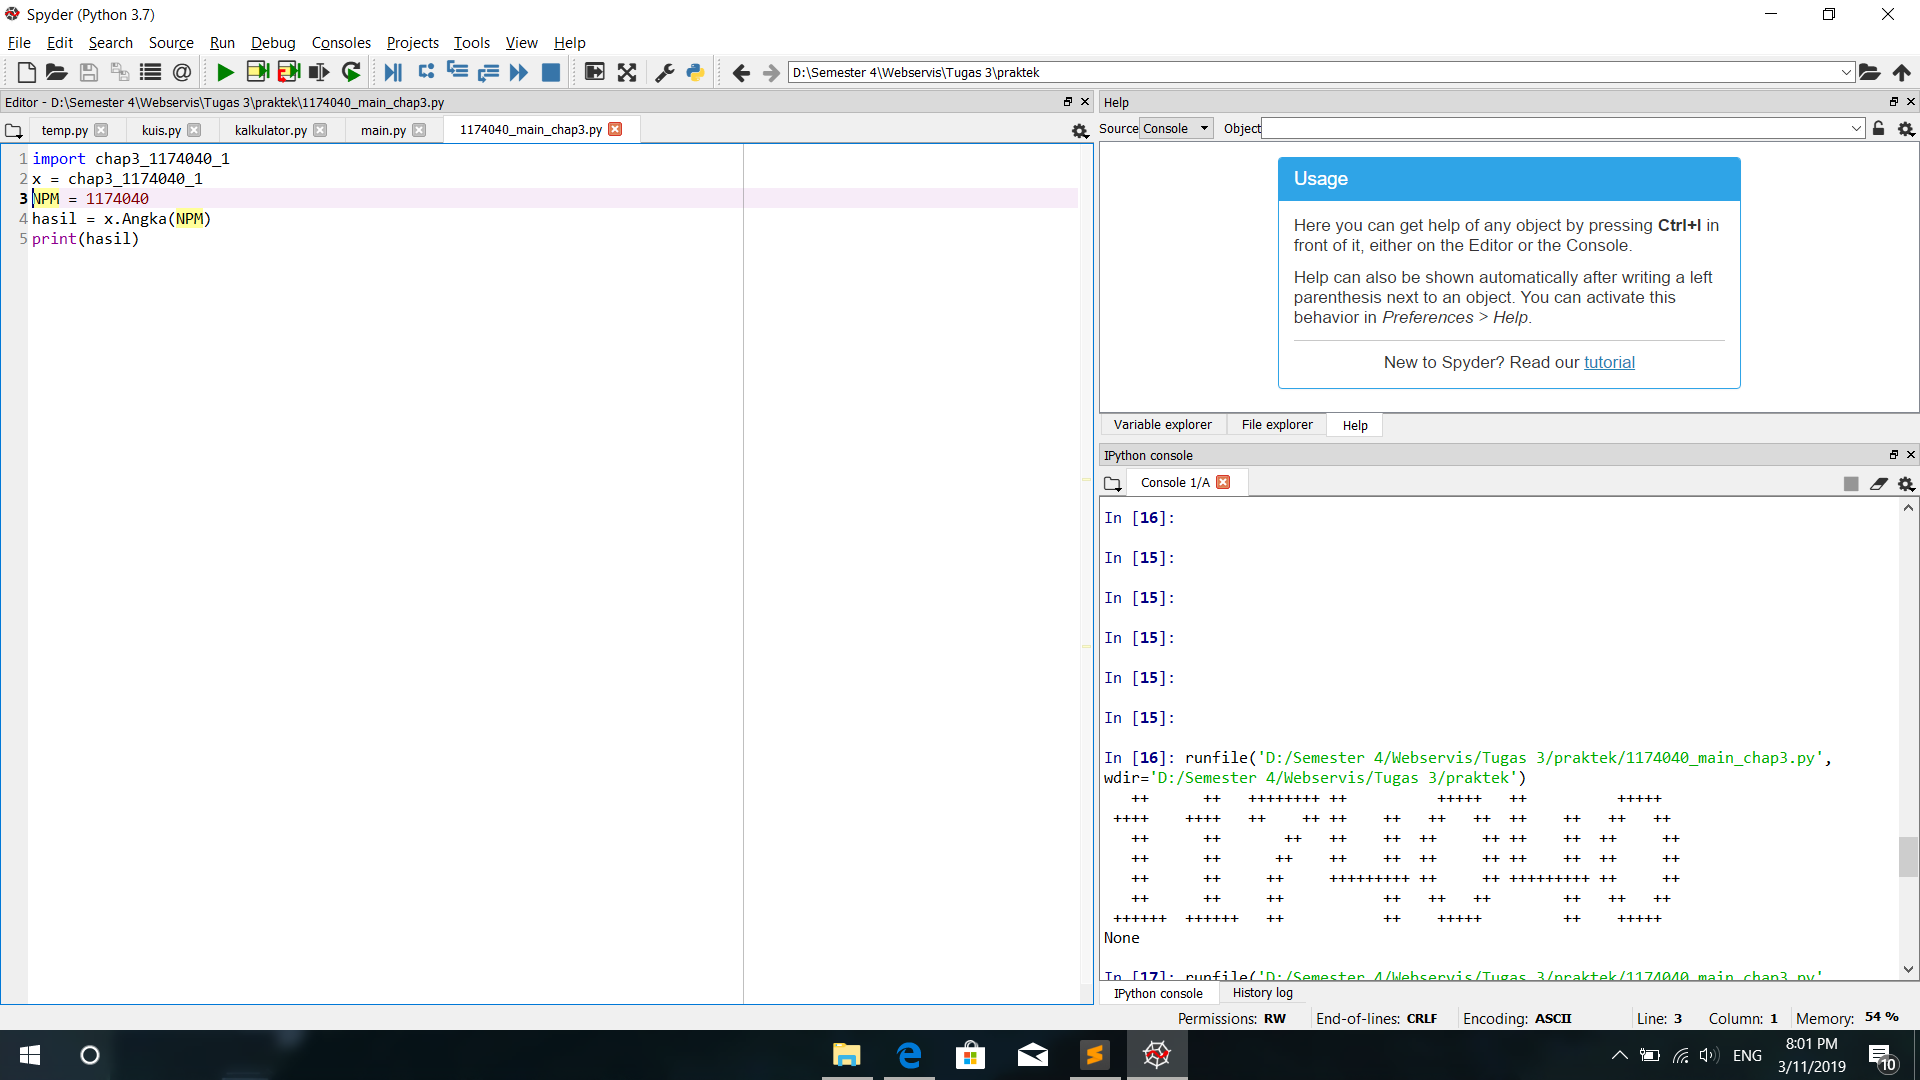
\includegraphics[width=0.5\textwidth]{figures/chapter3/1174040_1.png}}
            \caption{No. 1}
            \label{1174040_no1}
            \end{figure}

            \item \lstinputlisting{src/chapter3/chap3_1174040_2.py}
            \begin{figure}[ht]
            \centerline{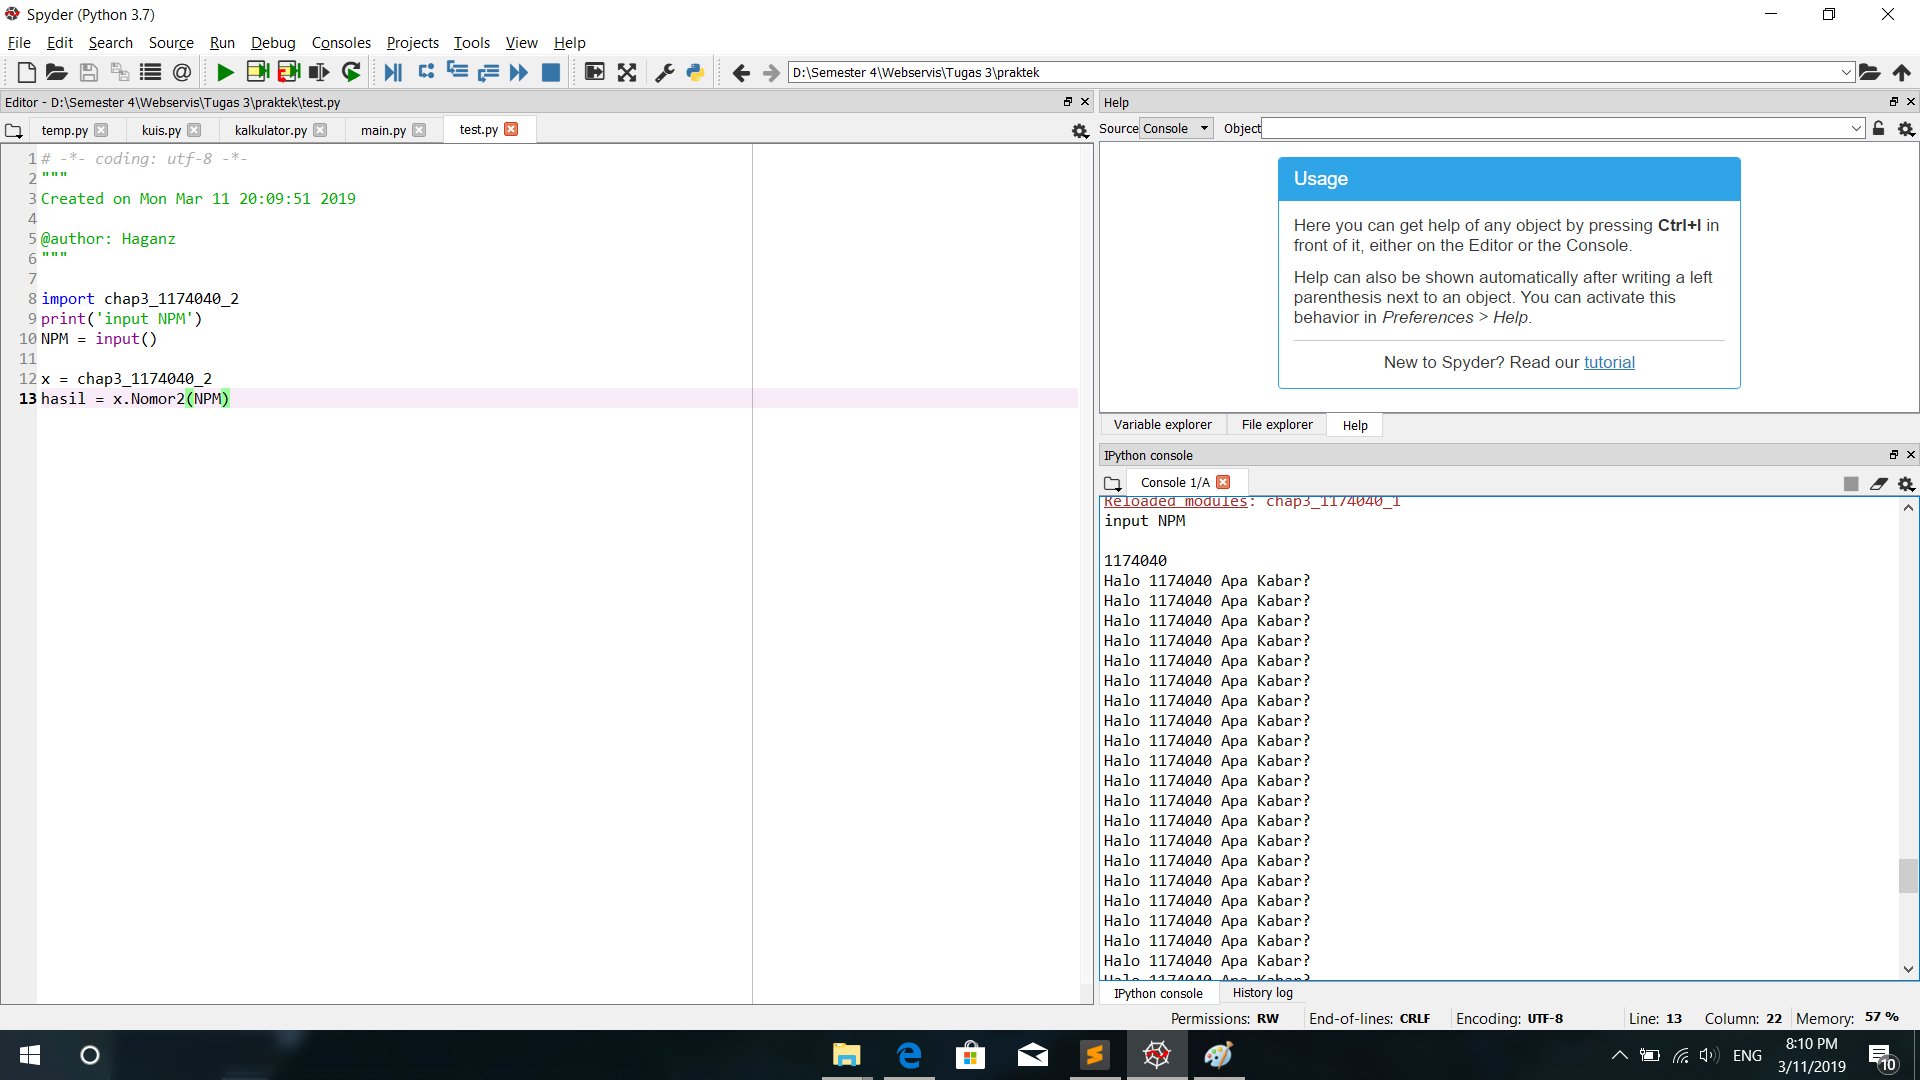
\includegraphics[width=0.5\textwidth]{figures/chapter3/1174040_2.png}}
            \caption{No. 2}
            \label{1174040_no2}
            \end{figure}

            \item \lstinputlisting{src/chapter3/chap3_1174040_3.py}
            \begin{figure}[ht]
            \centerline{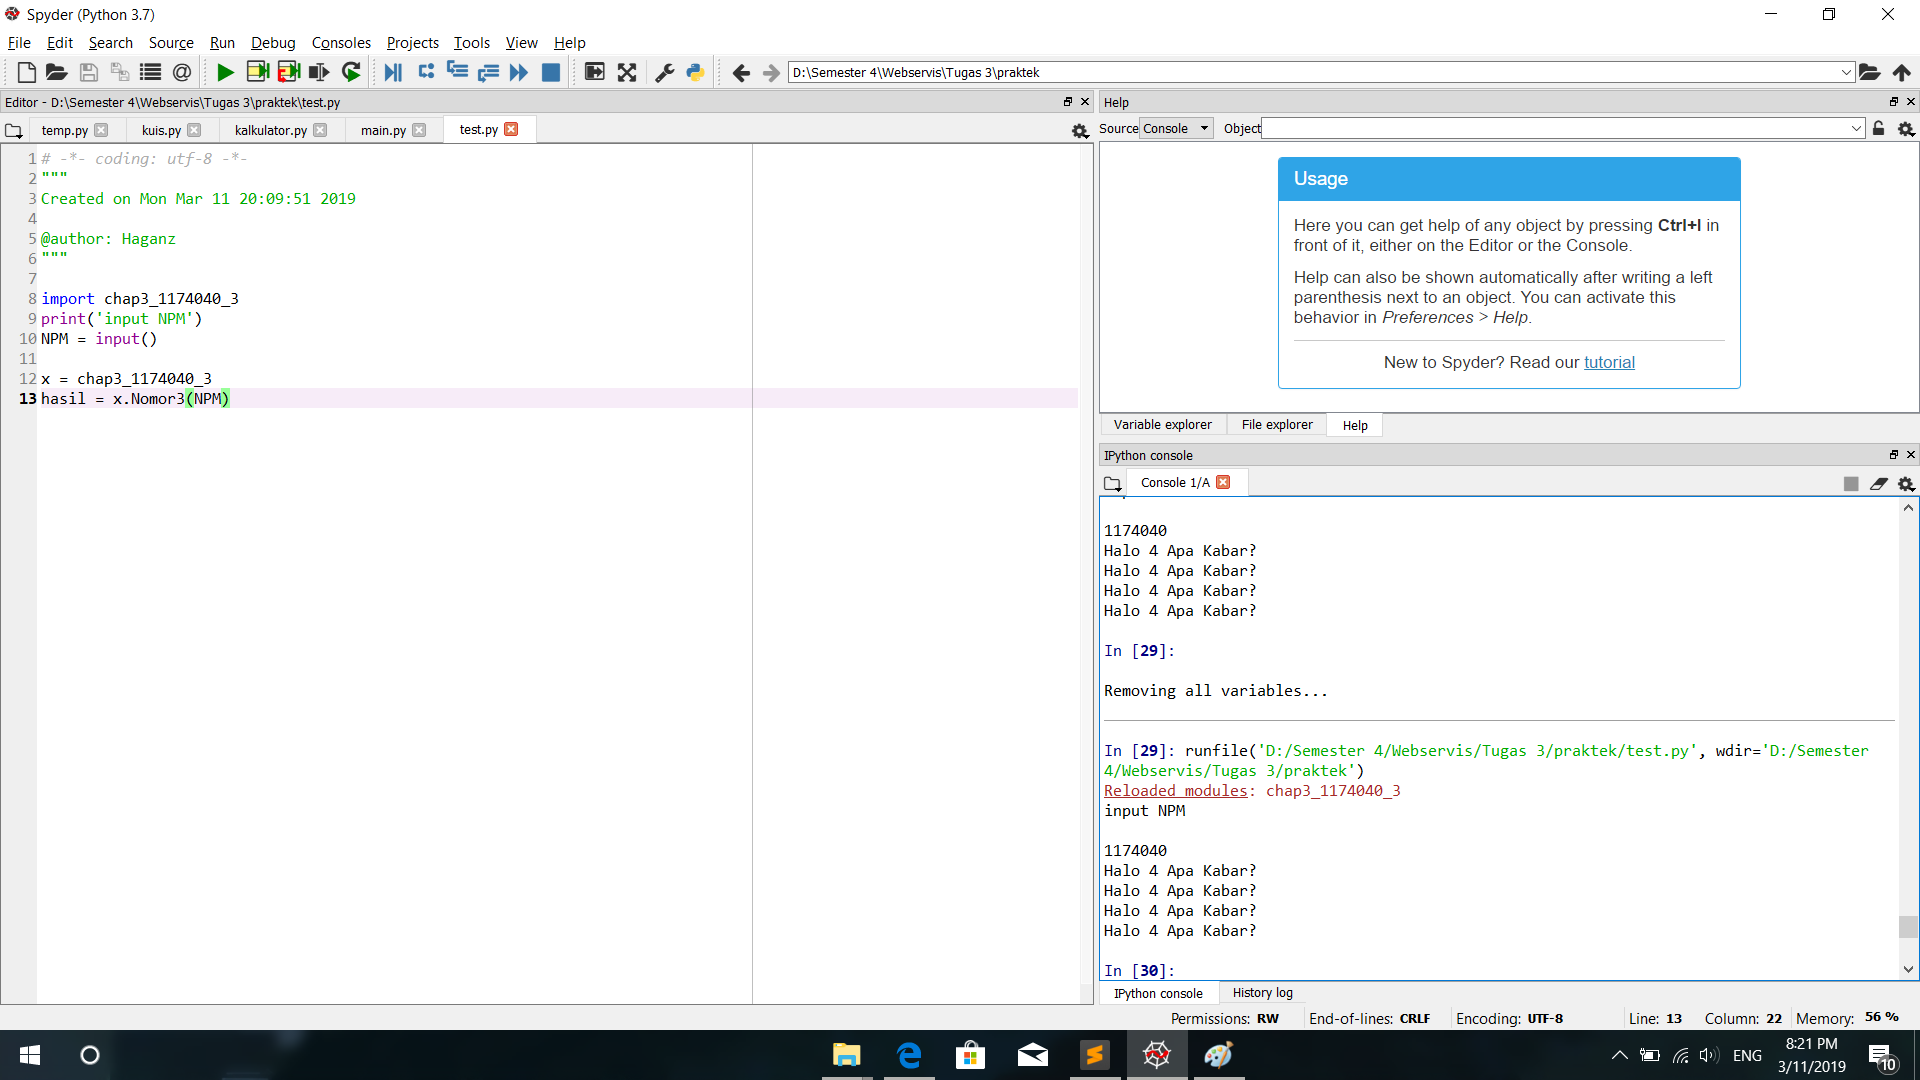
\includegraphics[width=0.5\textwidth]{figures/chapter3/1174040_3.png}}
            \caption{No. 3}
            \label{1174040_no3}
            \end{figure}

            \item \lstinputlisting{src/chapter3/chap3_1174040_4.py}
            \begin{figure}[ht]
            \centerline{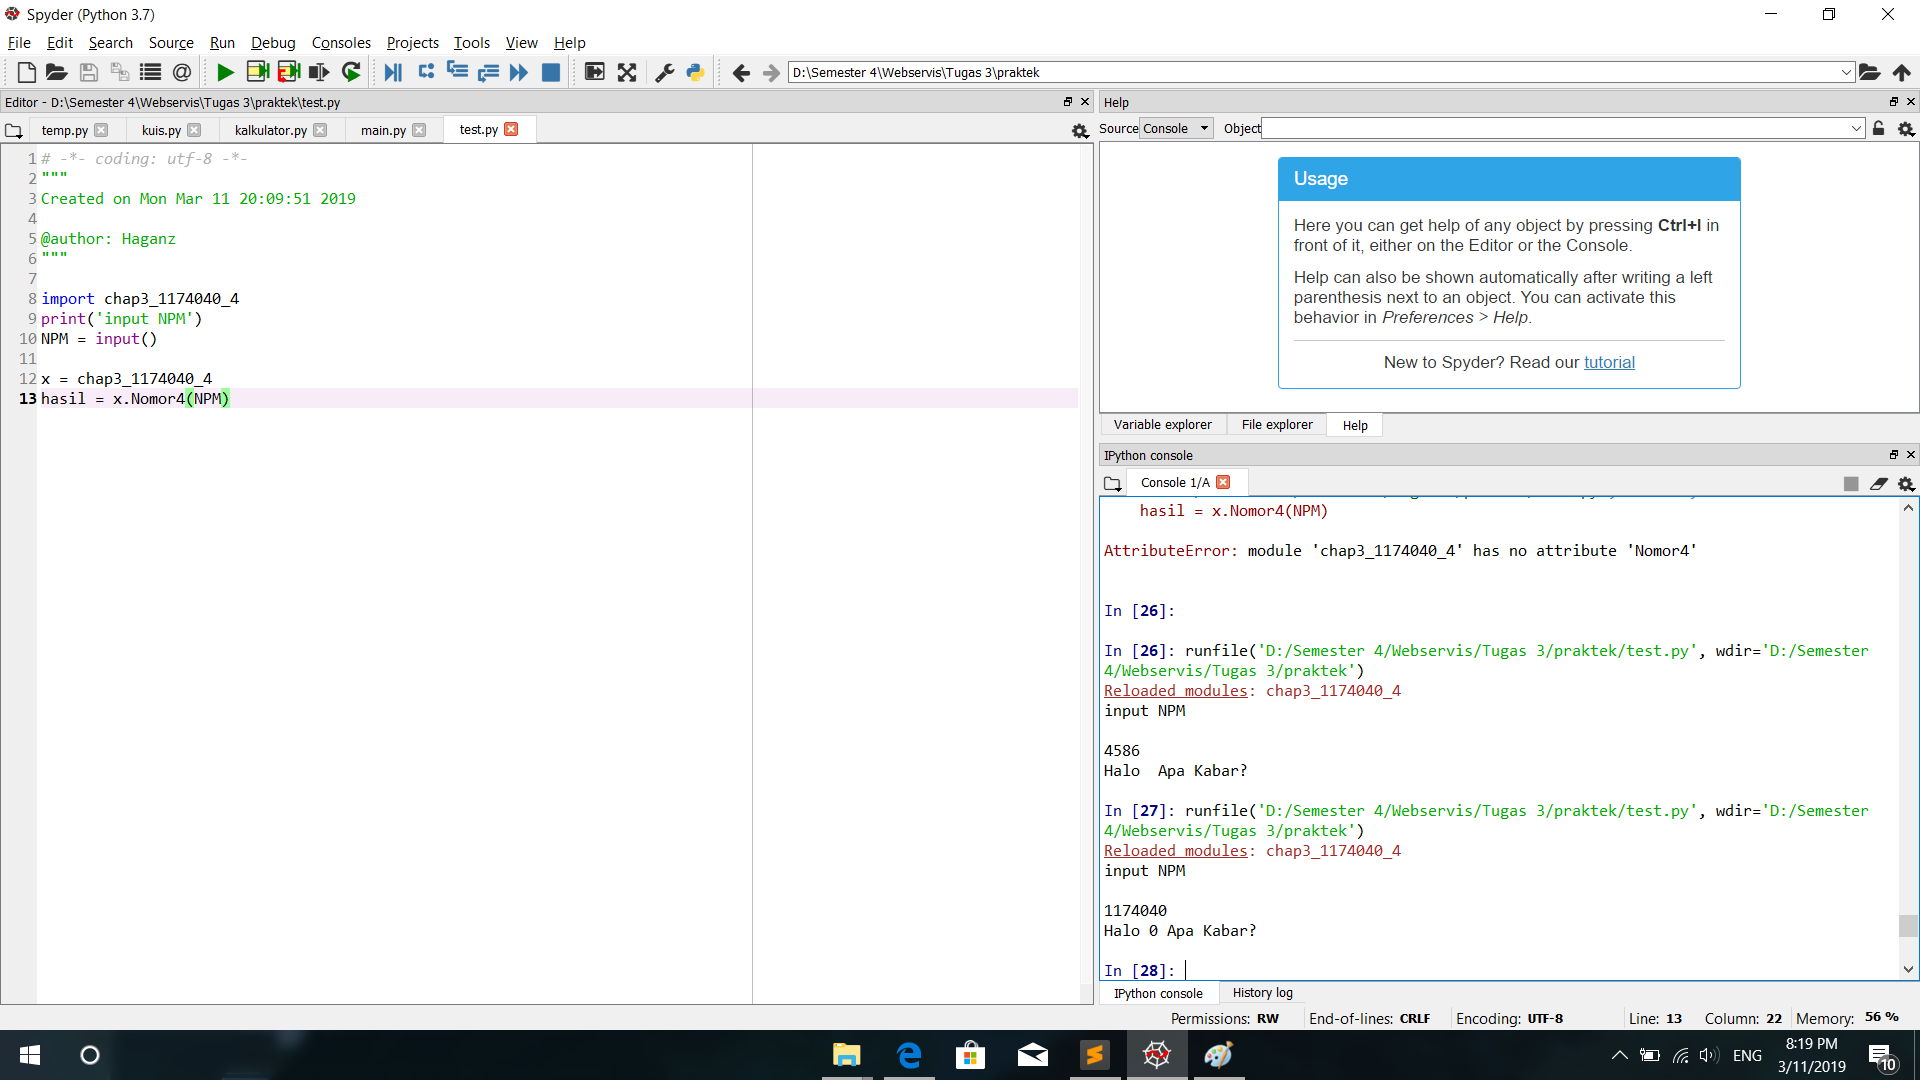
\includegraphics[width=0.5\textwidth]{figures/chapter3/1174040_4.png}}
            \caption{No. 4}
            \label{1174040_no4}
            \end{figure}

            \item \lstinputlisting{src/chapter3/chap3_1174040_5.py}
            \begin{figure}[ht]
            \centerline{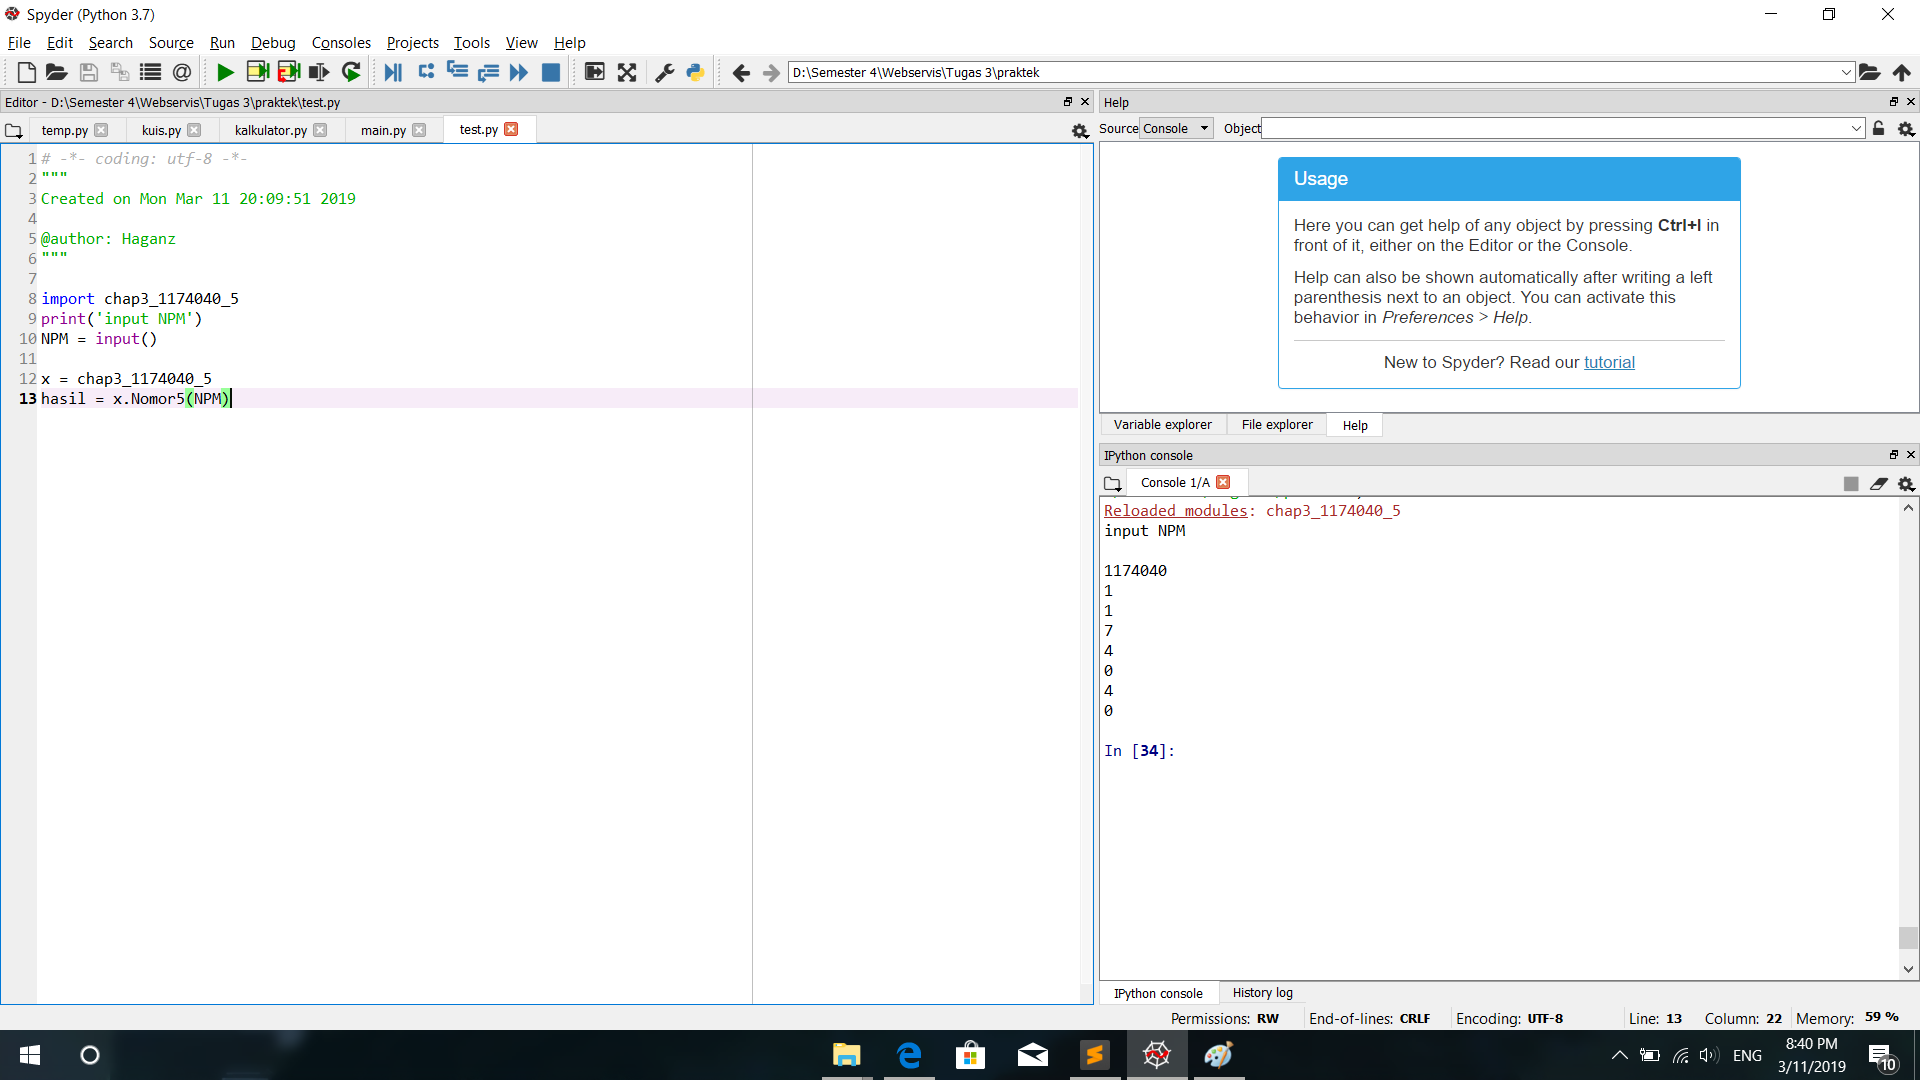
\includegraphics[width=0.5\textwidth]{figures/chapter3/1174040_5.png}}
            \caption{No. 5}
            \label{1174040_no5}
            \end{figure}

            \item \lstinputlisting{src/chapter3/chap3_1174040_6.py}
            \begin{figure}[ht]
            \centerline{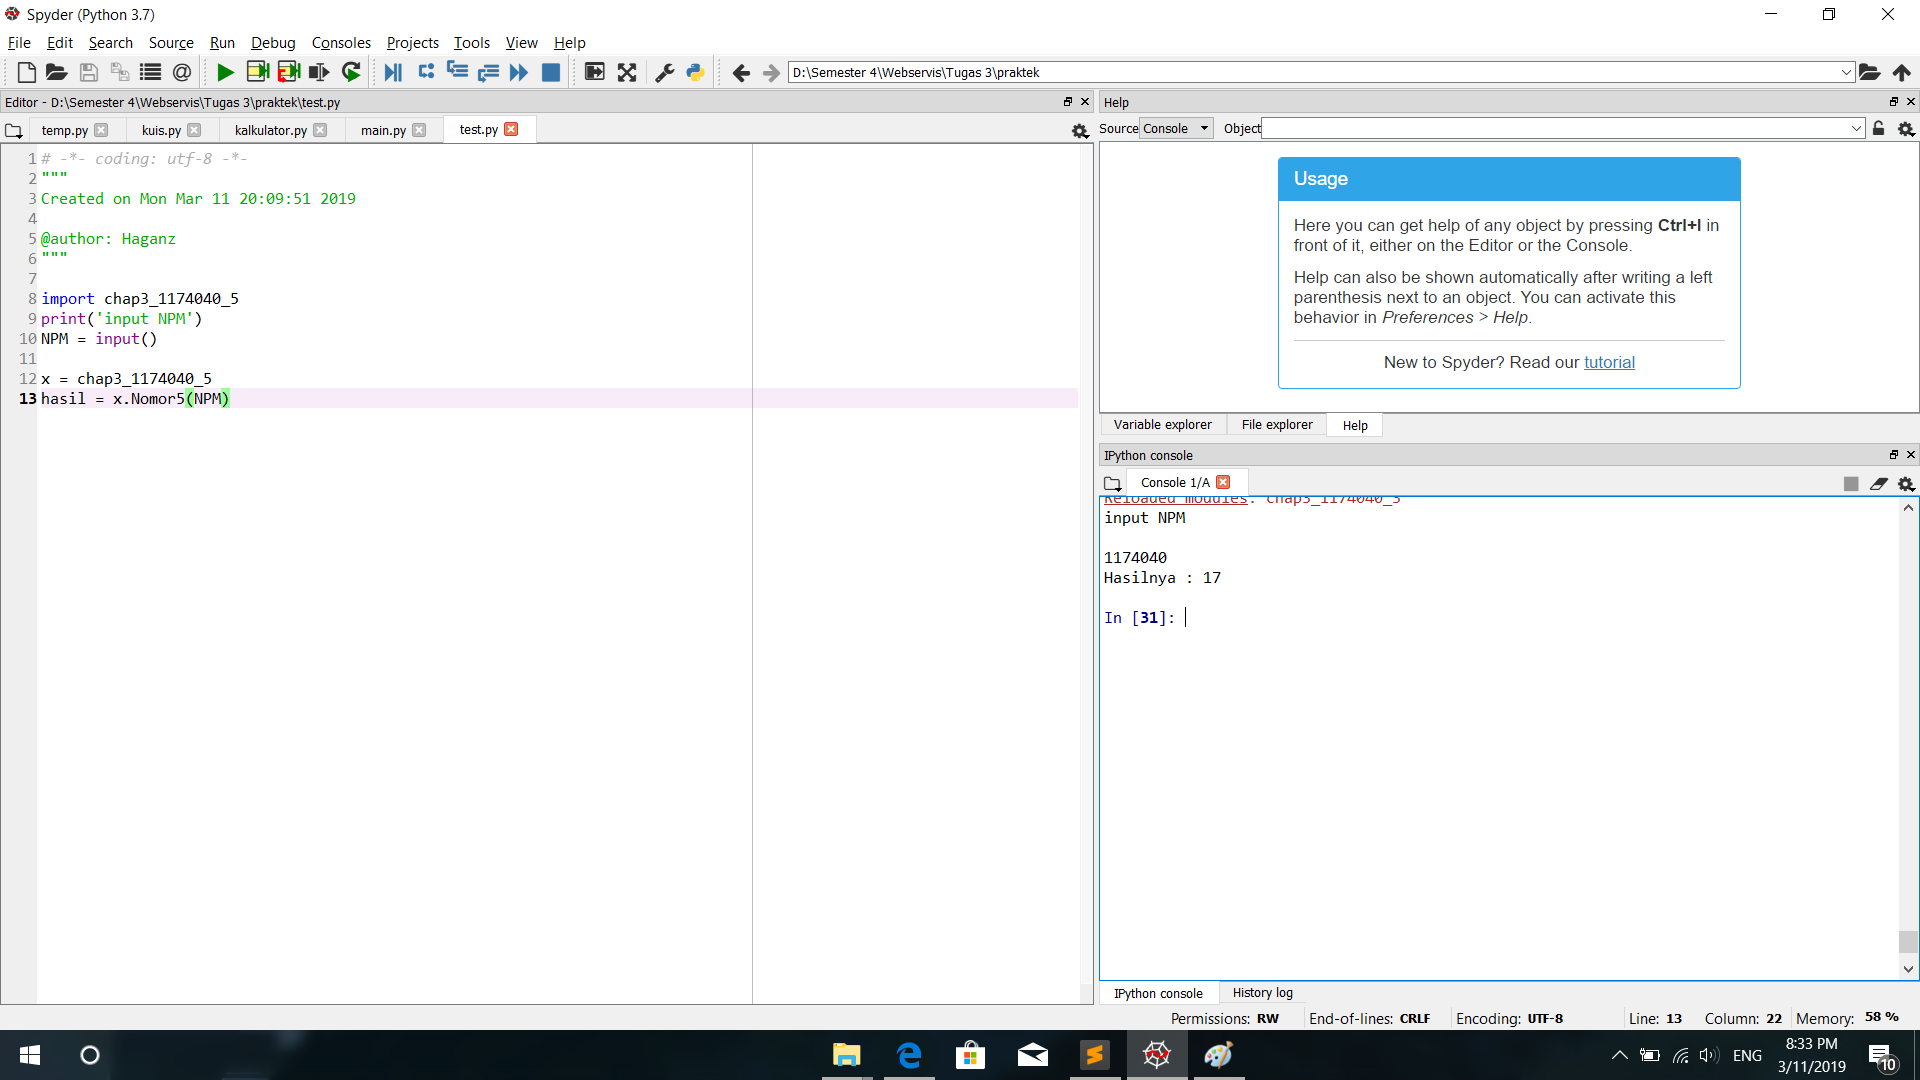
\includegraphics[width=0.5\textwidth]{figures/chapter3/1174040_6.png}}
            \caption{No. 6}
            \label{1174040_no6}
            \end{figure}

            \item \lstinputlisting{src/chapter3/chap3_1174040_7.py}
            \begin{figure}[ht]
            \centerline{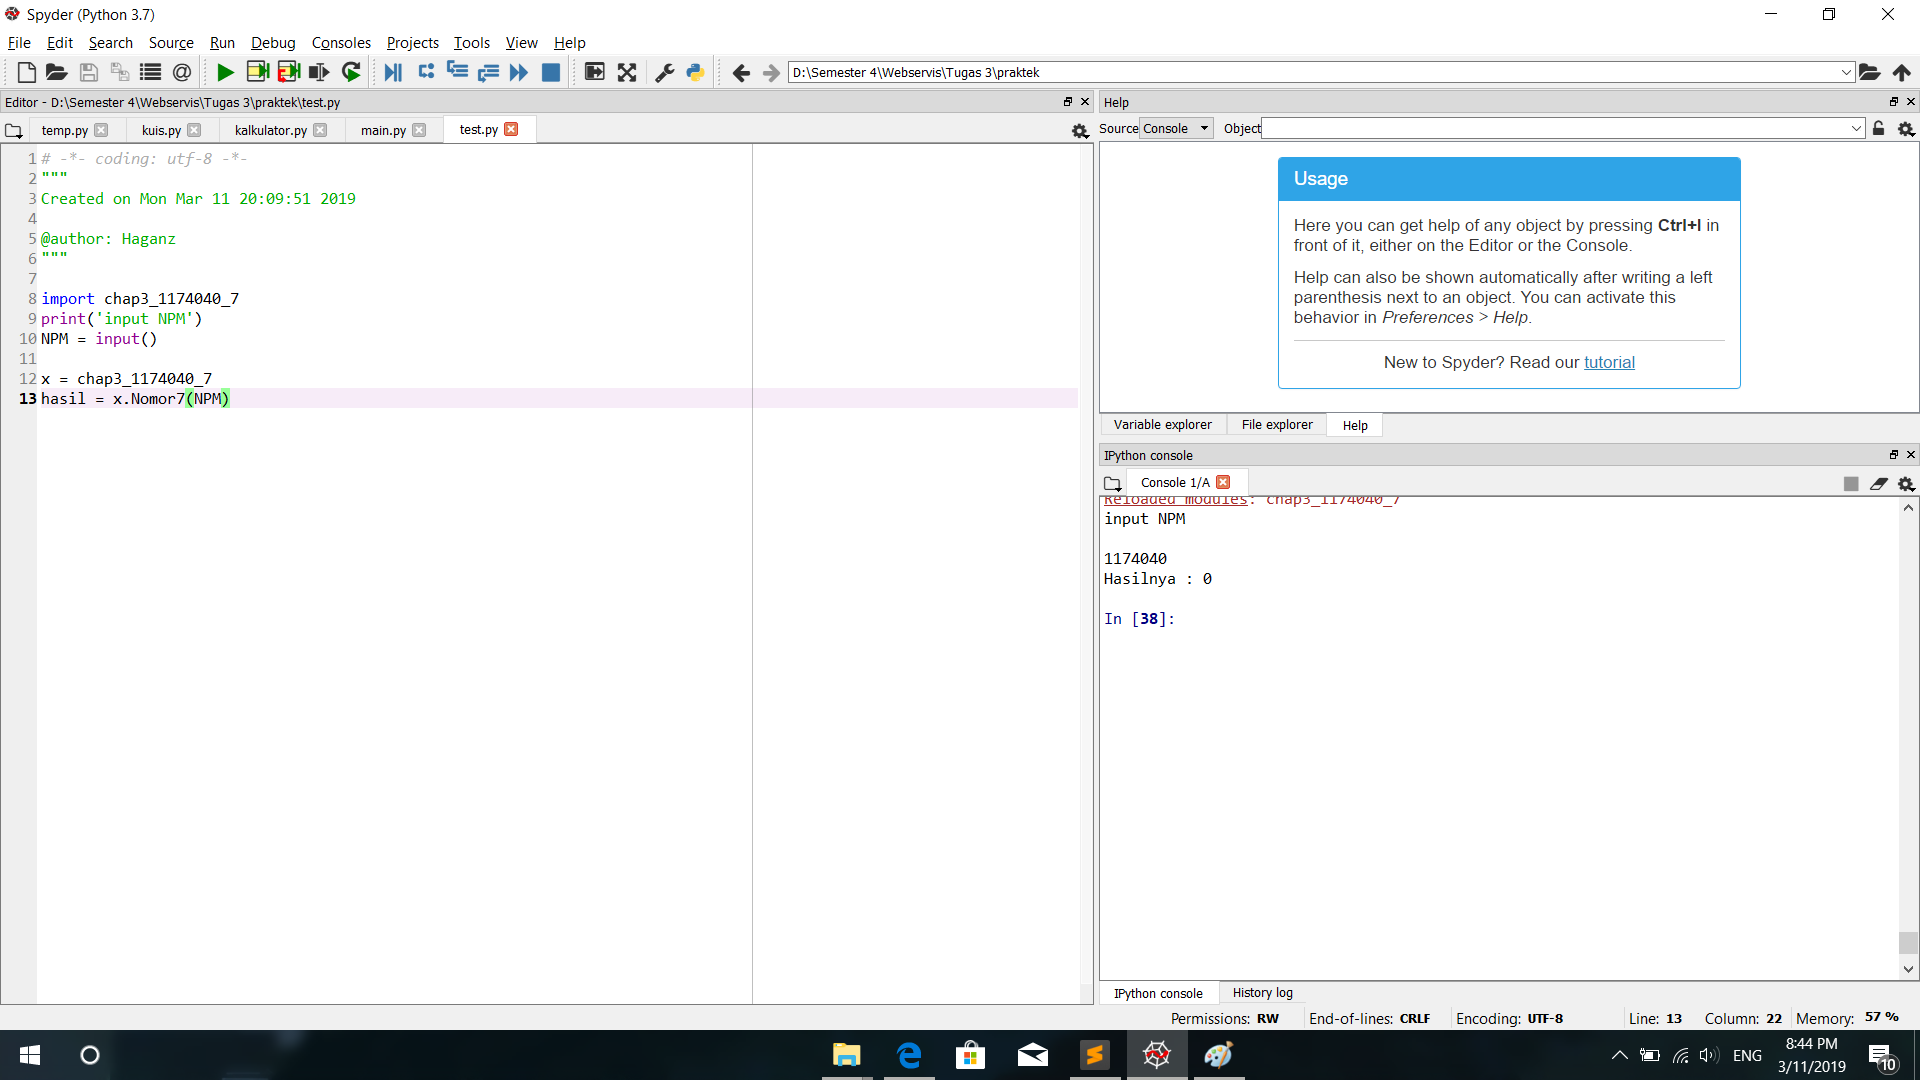
\includegraphics[width=0.5\textwidth]{figures/chapter3/1174040_7.png}}
            \caption{No. 7}
            \label{1174040_no7}
            \end{figure}

            \item \lstinputlisting{src/chapter3/chap3_1174040_8.py}
\begin{figure}[ht]

            \centerline{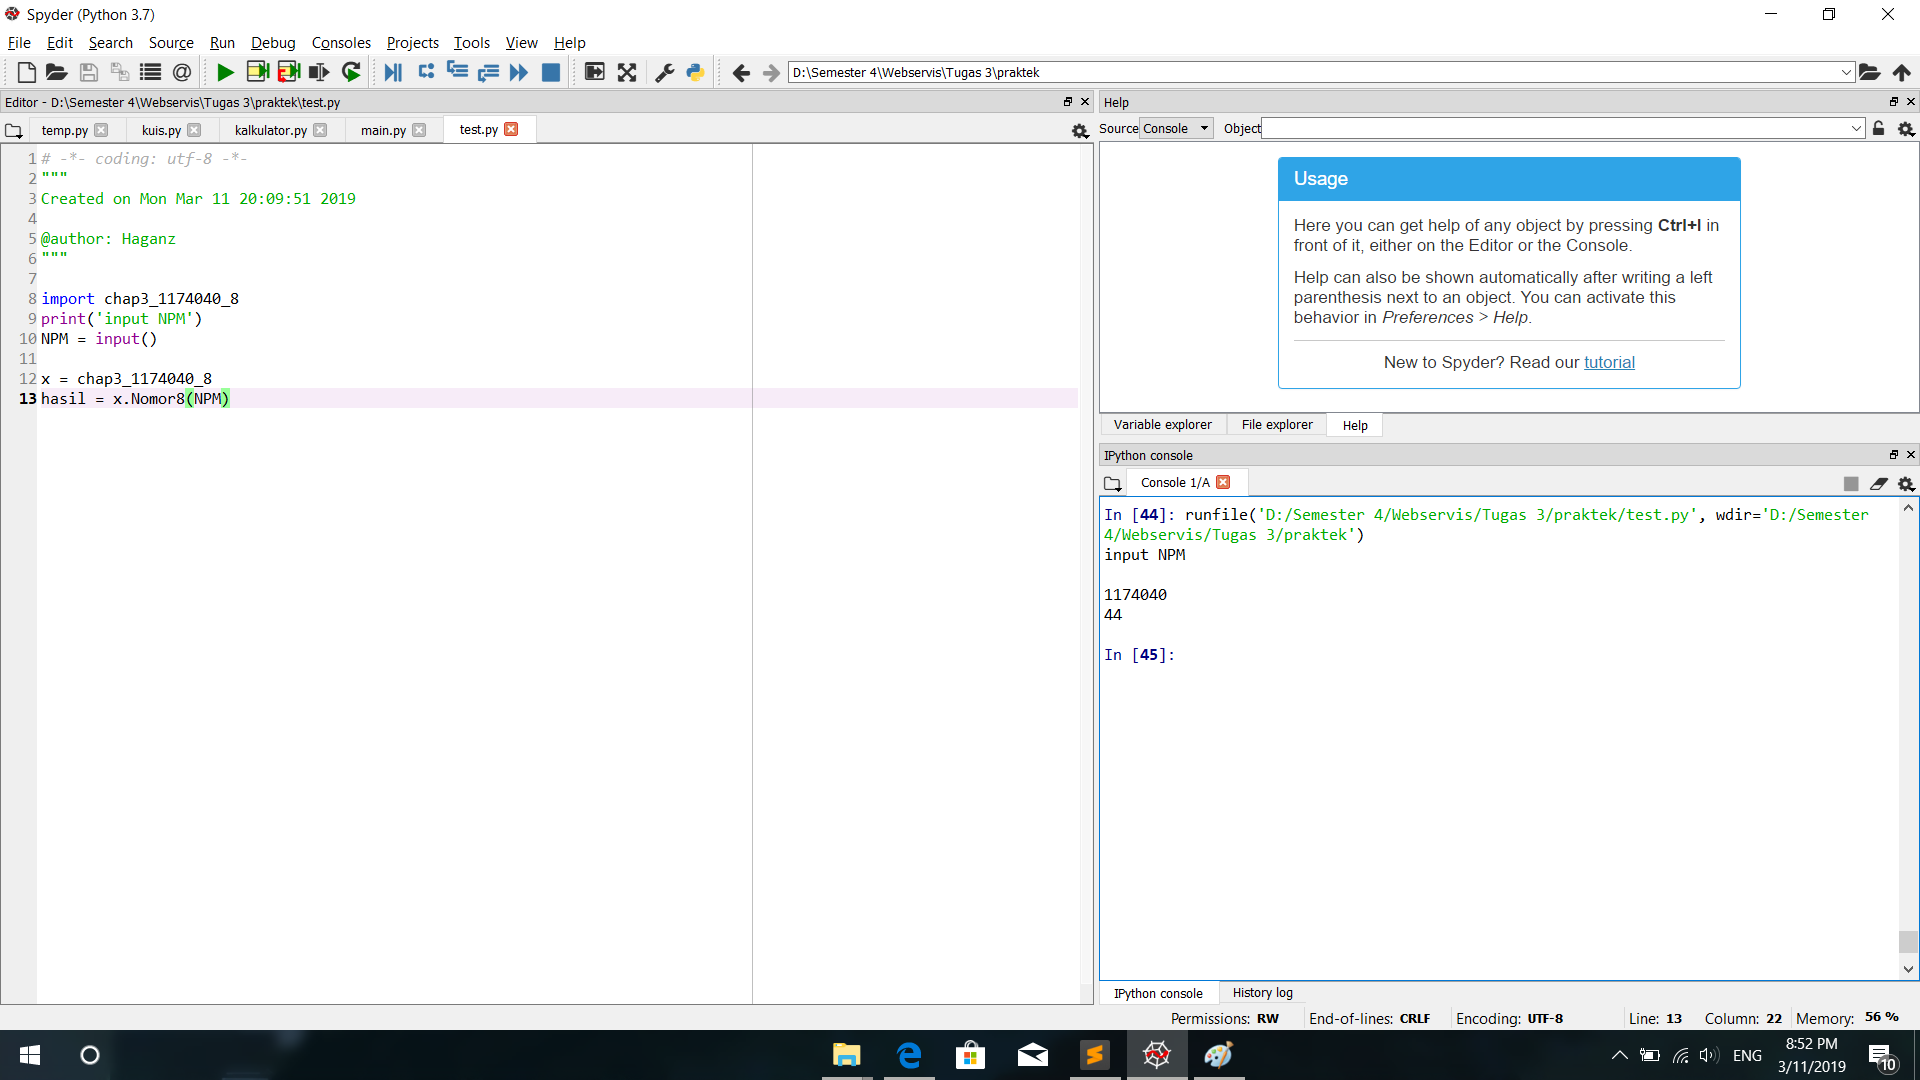
\includegraphics[width=0.5\textwidth]{figures/chapter3/1174040_8.png}}

            \caption{Gambar 8}

            \label{1174040_8}

            \end{figure}

            \item \lstinputlisting{src/chapter3/chap3_1174040_9.py}

\begin{figure}[ht]
            \centerline{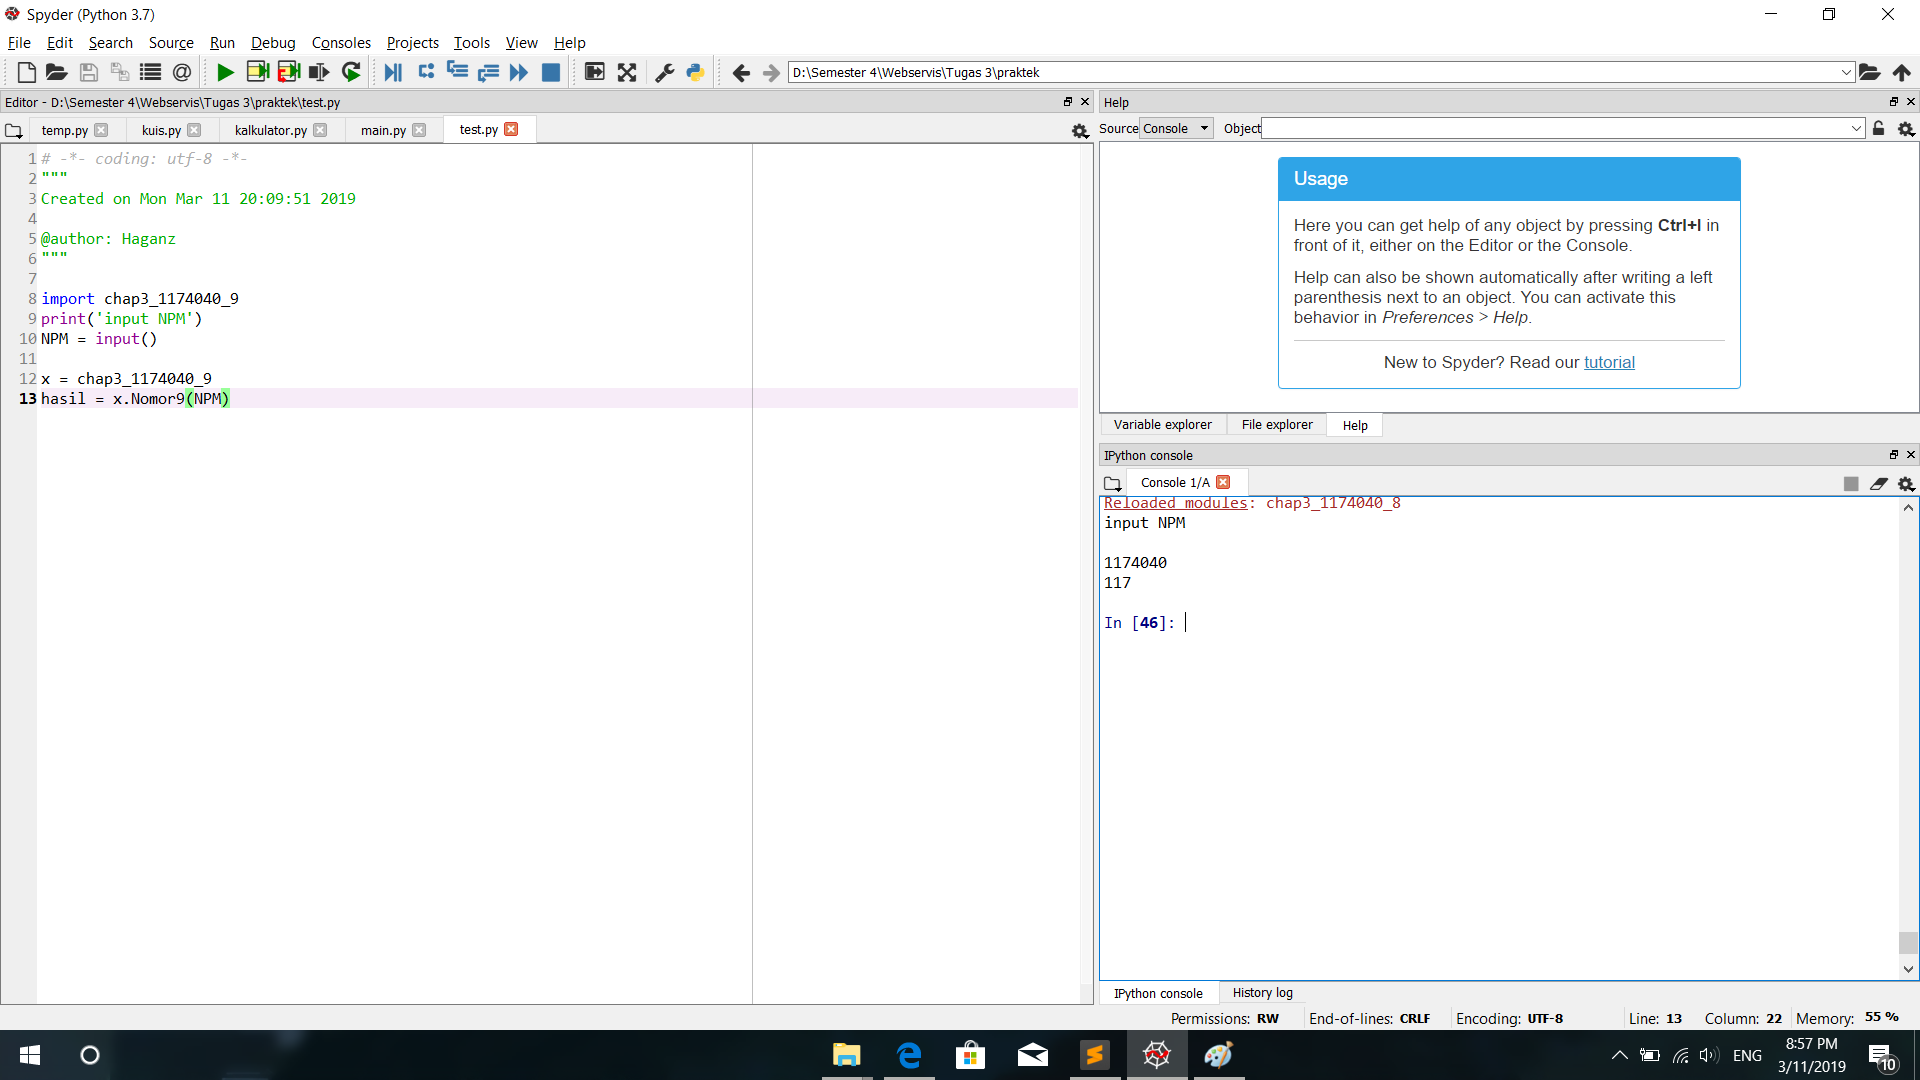
\includegraphics[width=0.5\textwidth]{figures/chapter3/1174040_9.png}}
            \caption{No. 9}
            \label{1174040_no9}
            \end{figure}

            \item \lstinputlisting{src/chapter3/chap3_1174040_10.py}

            \begin{figure}[ht]

            \centerline{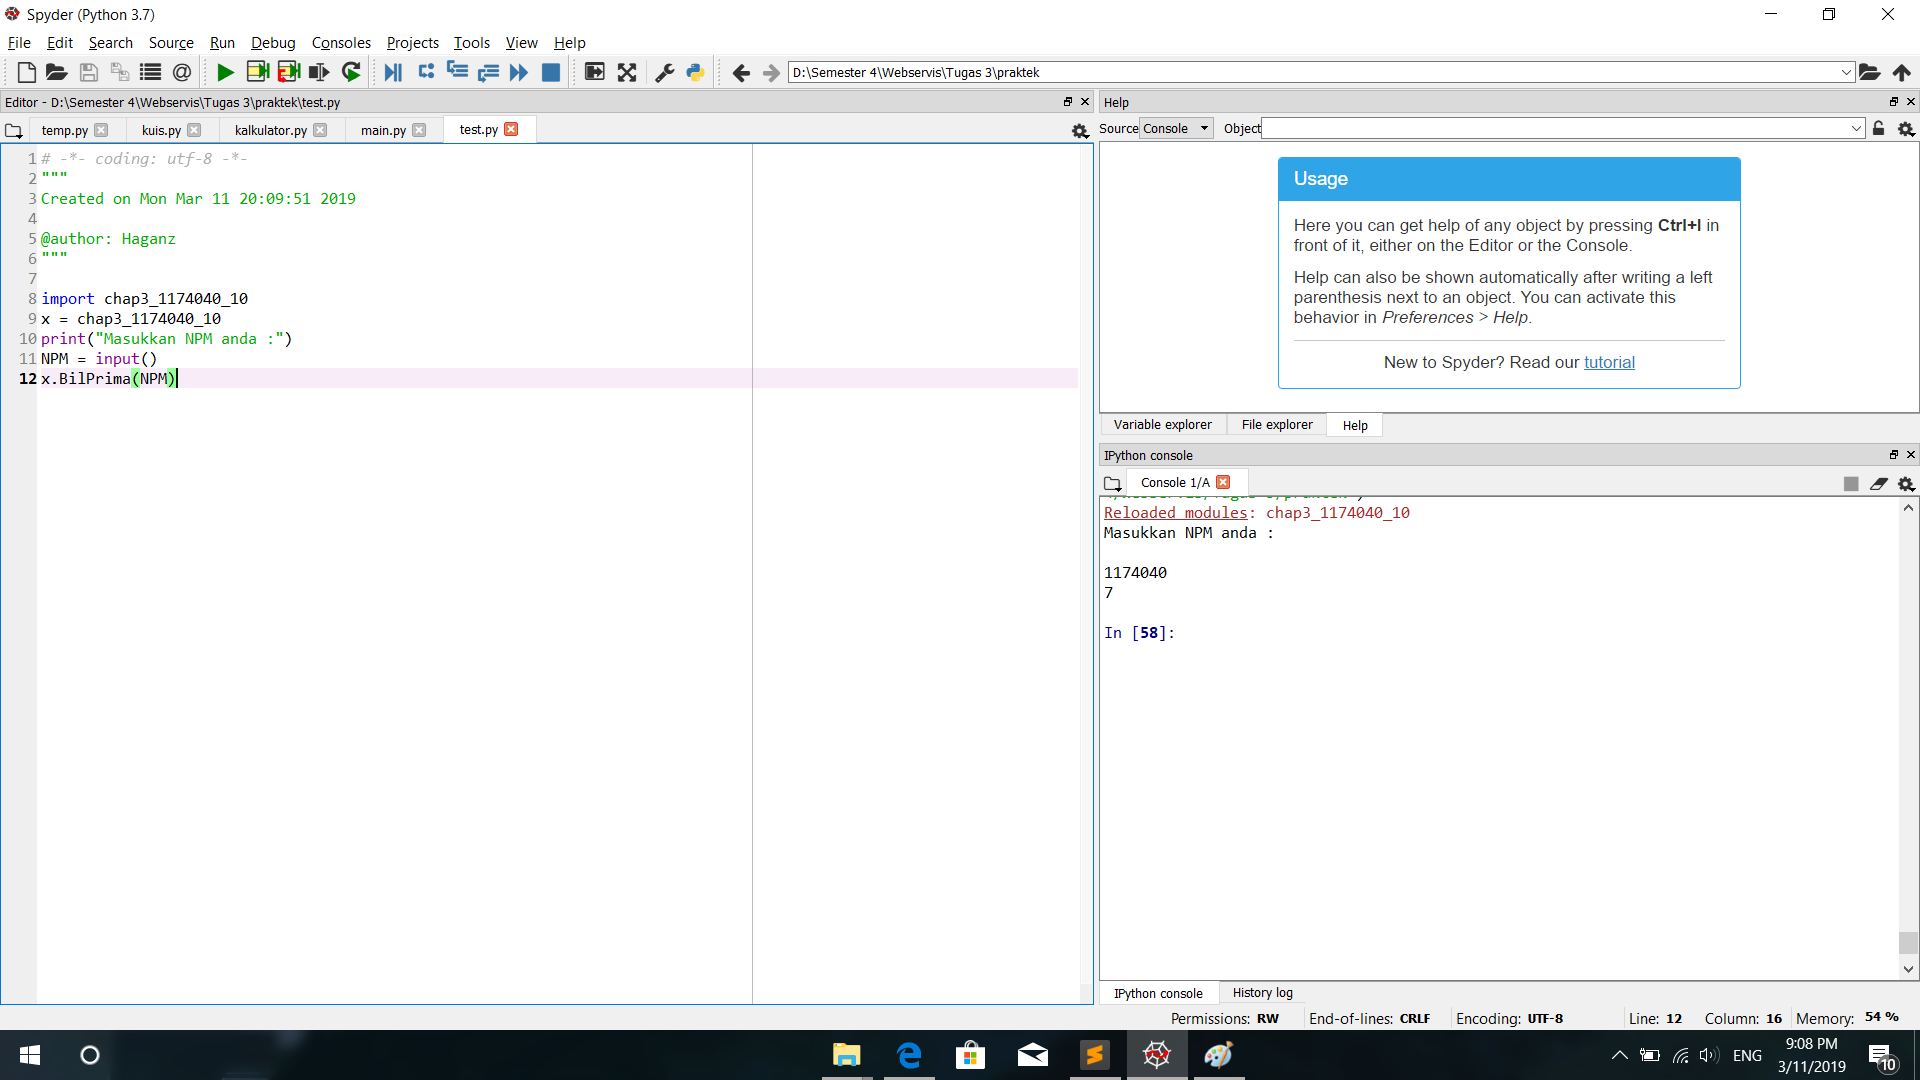
\includegraphics[width=0.5\textwidth]{figures/chapter3/1174040_10.png}}
            \caption{No. 10}
            \label{1174040_no10}
            \end{figure}

            \item Membuat library 3lib.py dan memanggilnya di main.py
            \lstinputlisting[firstline=2, lastline=7]{src/chapter3/chap3_1174040_main.py}
            \begin{figure}[ht]

            \centerline{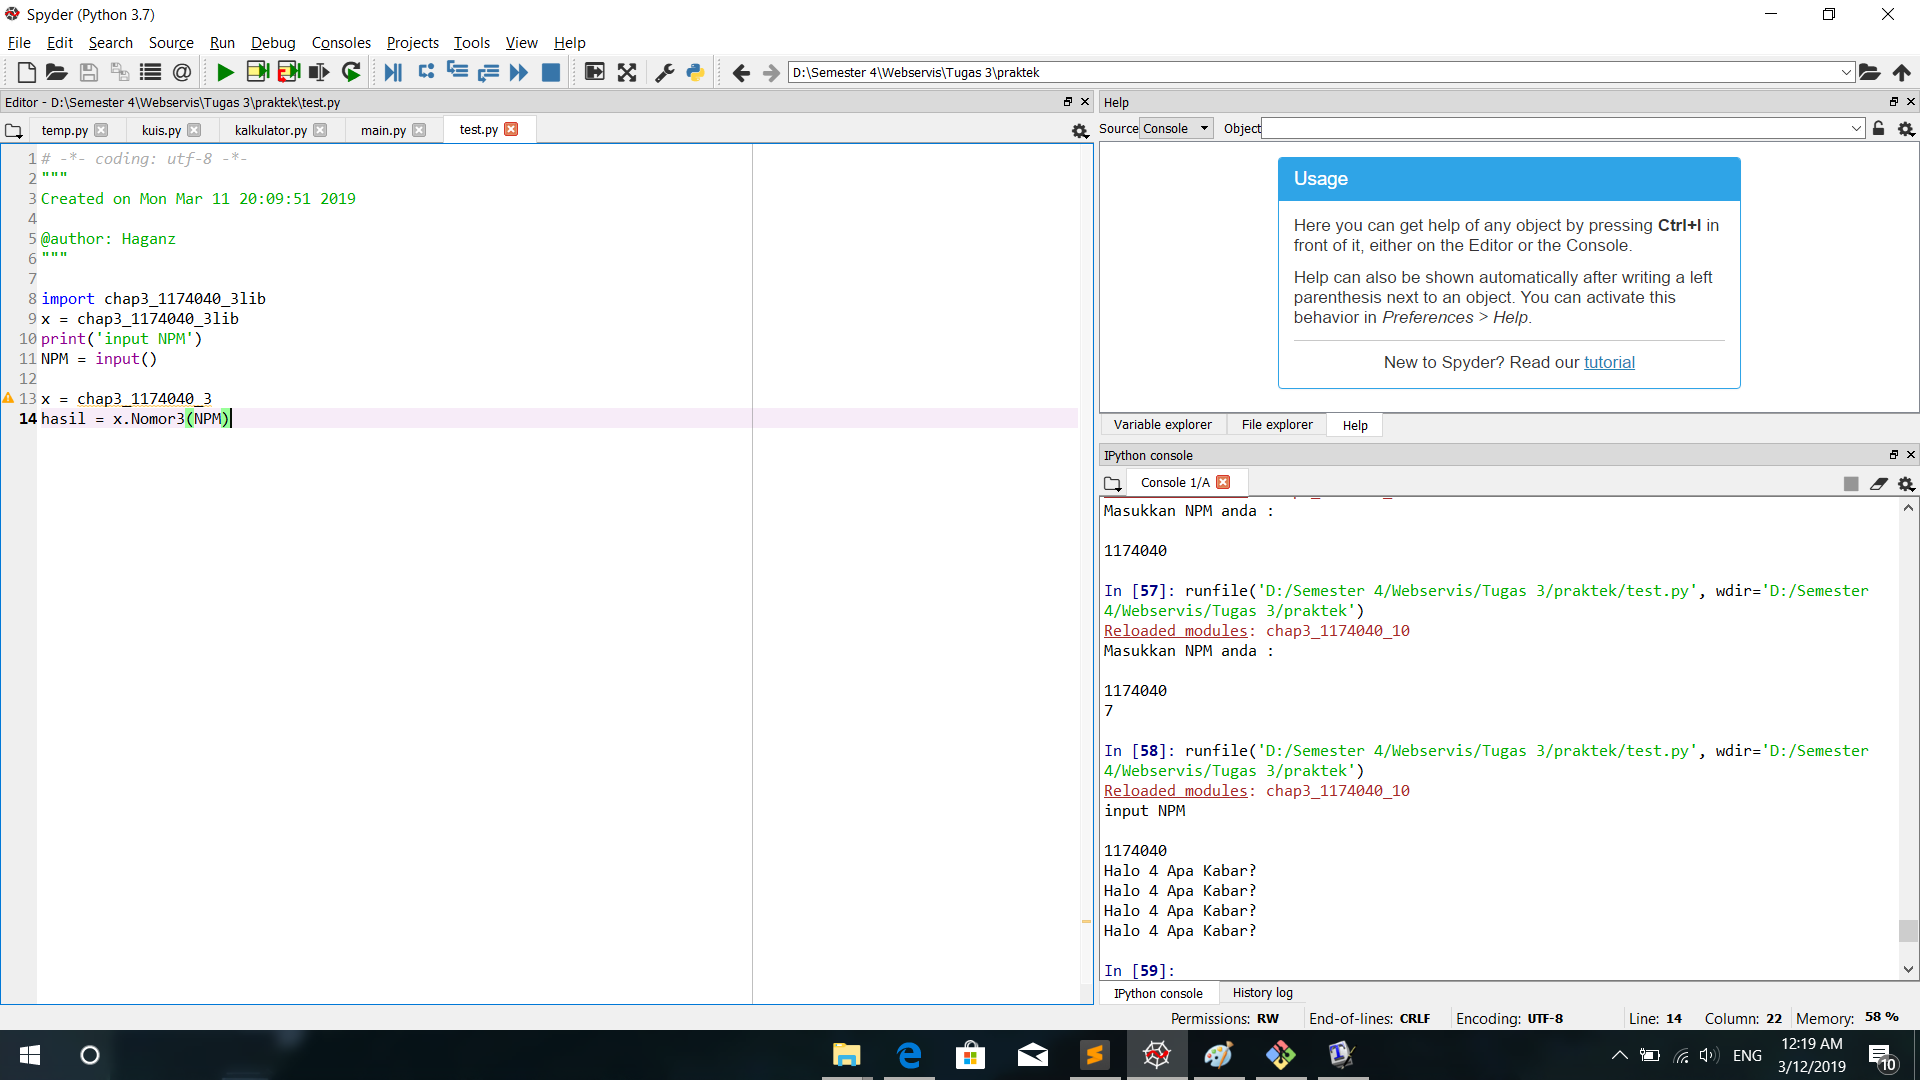
\includegraphics[width=0.5\textwidth]{figures/chapter3/1174040_11.png}}
            \caption{No. 11}
            \label{1174040_no11}
            \end{figure}

            \item Membuat library kelas dengan nama kelas3lib.py yang merupakan modifikasi dari fungsi - fungsi diatas dan berikan contoh pemanggilannya di main.py
            \lstinputlisting[firstline=10, lastline=14]{src/chapter3/chap3_1174040_main.py}
            \begin{figure}[ht]

            \centerline{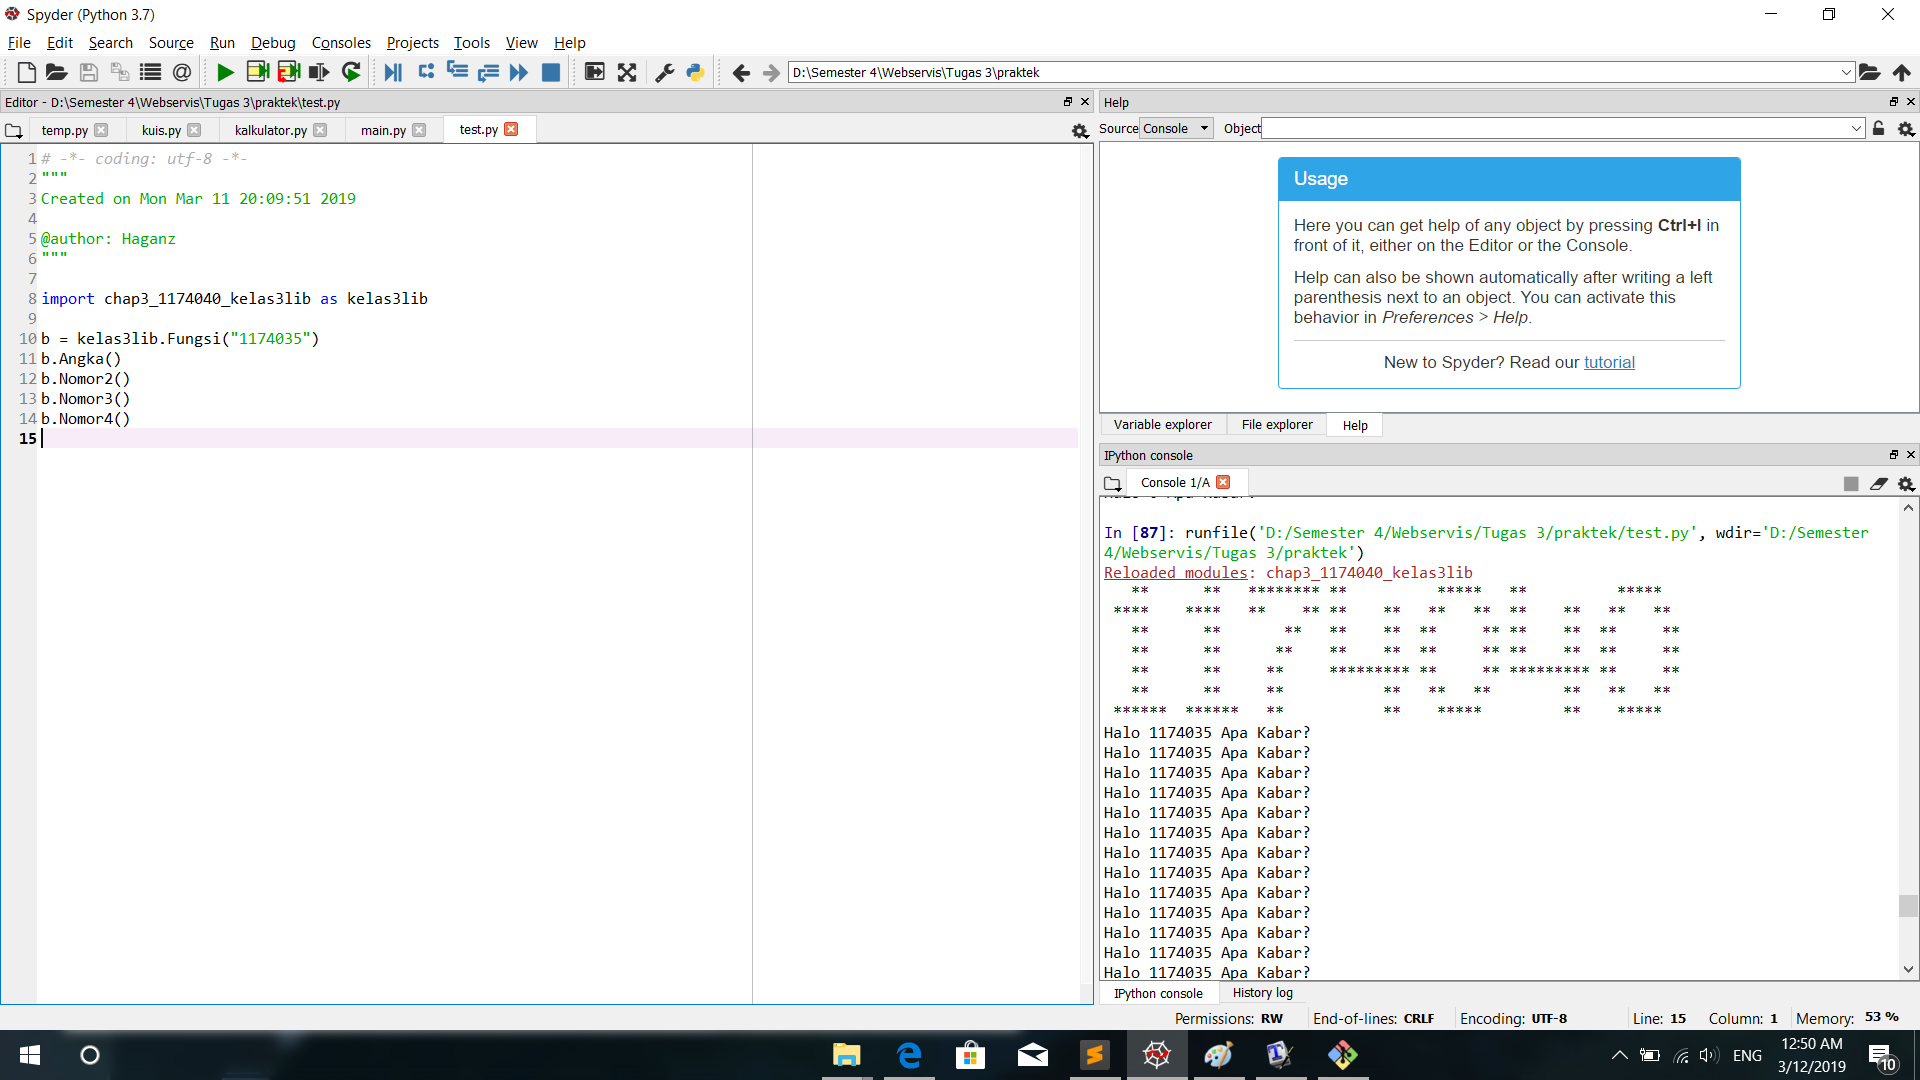
\includegraphics[width=0.5\textwidth]{figures/chapter3/1174040_12.png}}
            \caption{No. 12}
            \label{1174040_no12}
            \end{figure}

        \end{enumerate}
    \subsection{Keterampilan Penanganan Error}
        \begin{enumerate}
            \item Type error karena hasil dari input() adalah string jadi jika masuk kedalam perhitungan dan perbandingan, harus terlebih dahulu diubah menjadi tipe data integer.
            Contoh try dan catch adalah :

            \lstinputlisting{src/chapter3/chap3_1174040_3err.py}
        \end{enumerate}
    \subsection{Cek Plagiarisme}
    \begin{figure}[ht]

            \centerline{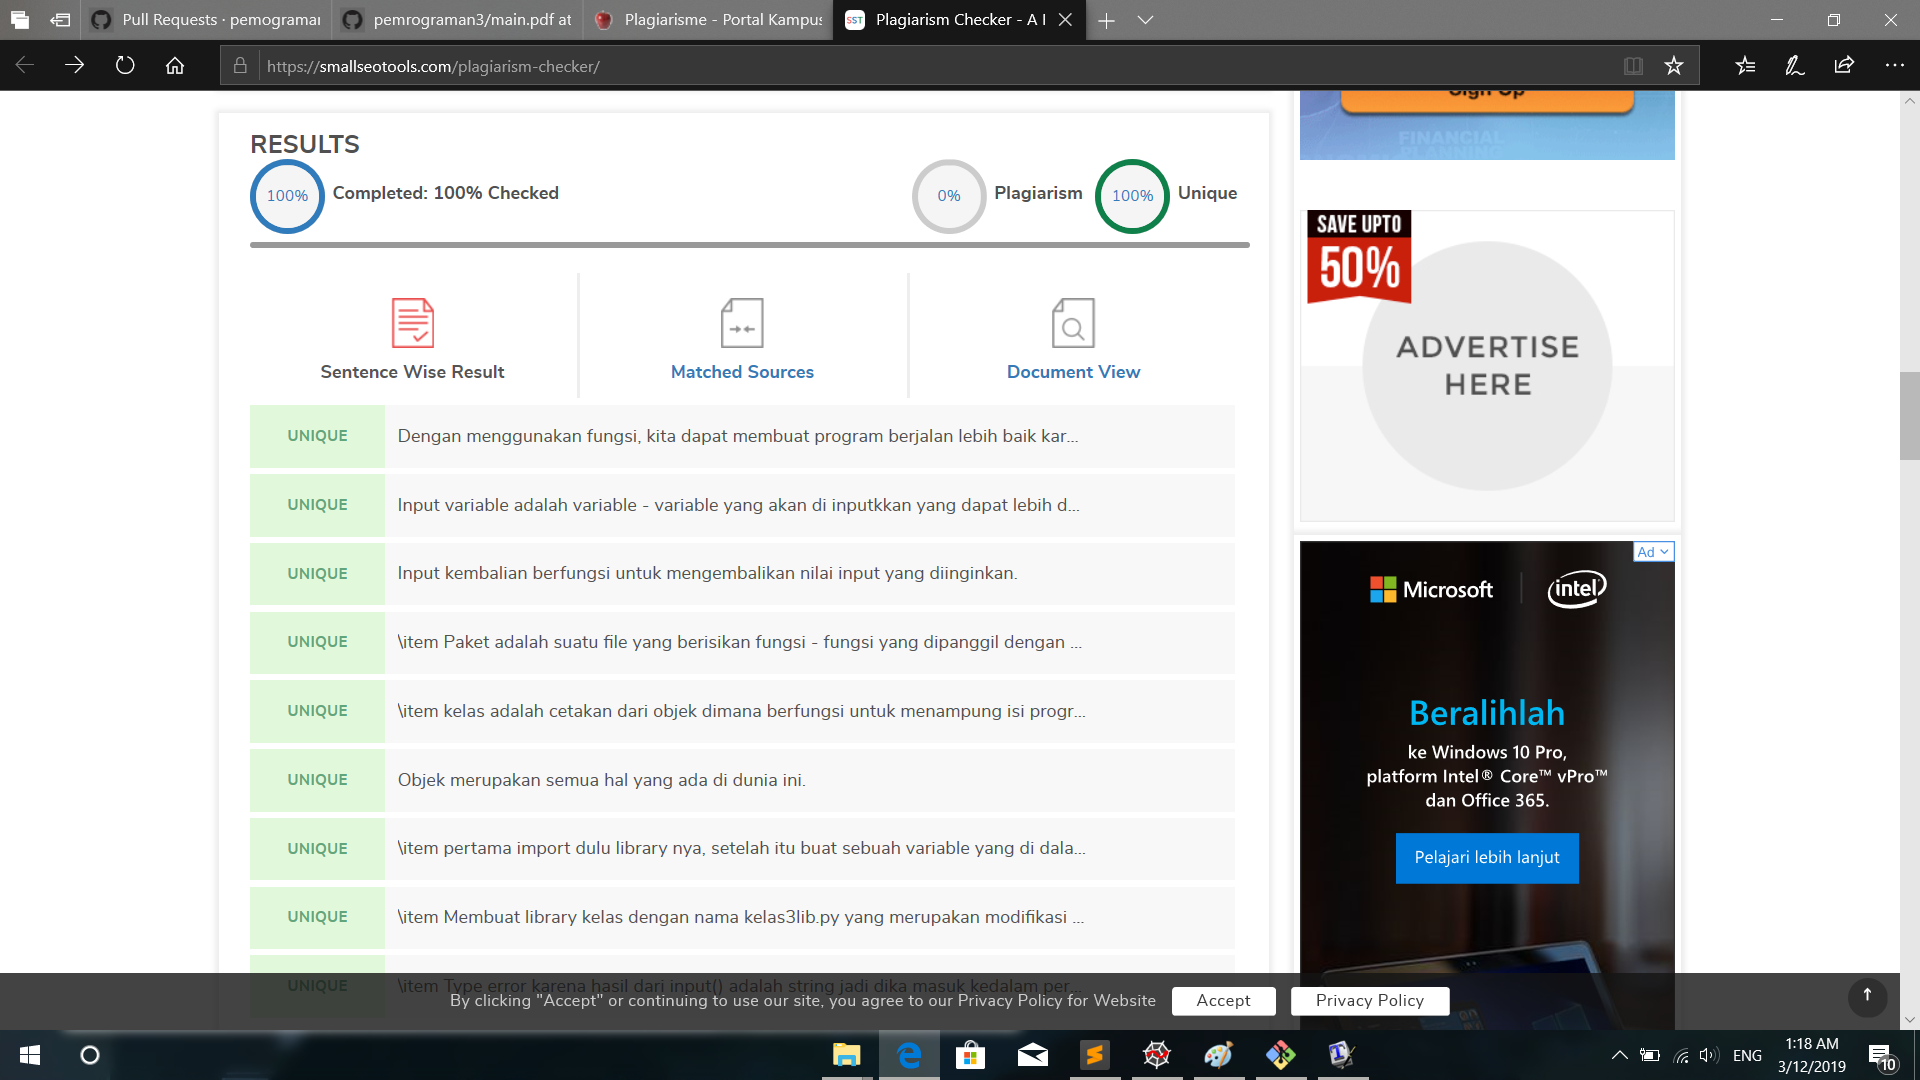
\includegraphics[width=0.5\textwidth]{figures/chapter3/1174040_plagiat.png}}
            \caption{Cek Plagiarisme}
            \label{1174040_cekplagiat}
            \end{figure}

\section{IrvanRizkiansyah/1174043}
	\subsection{Pemahaman Teori}
		\begin{enumerate}
			\item	\begin{itemize}
						\item Fungsi adalah bagian dari program yang berupa blok kode yang diberikan nama dan nama tersebut berguna untuk memanggil fungsi tersebut.
					
						\item Inputan fungsi adalah sebuah fungsi yang telah di sediakan pada library python, yang berguna untuk menerima inputan dari user.
					
						\item Kembalian fungsi adalah sebuah nilai balikan yang diberikan oleh sebuah fungsi yang dibuat.
					\end{itemize}
					
					Contoh Program : 
					\lstinputlisting[language=Python, firstline=2, lastline=8]{src/chapter3/teori_1174043_chap3.py}
					
			\item paket adalah sebuah cara yang dilakukan untuk memanggil file script python, yang nantinya akan digunakan fungsi fungsi yang terdapat pada file script yang dipanggil tersebut. cara pemanggilan paket dengan cara :
				\begin{verbatim}
				import scriptFilePython
				\end{verbatim}
			
			Contoh Program :
			\lstinputlisting[language=Python, firstline=11, lastline=11]{src/chapter3/teori_1174043_chap3.py}
			
			\item	\begin{itemize}
						\item Kelas merupakan sebuah cetakan atau Blueprint yang berguna untuk mencetak objek.
						
						\item Objek merupakan sebuah objek yang dari proses hasil dari cetakan atau blueprint.
						
						\item Atribut merupakan penggambaran data yang bisa memberikan sebuah informasi kelas atau objek dimana atribut tersebut berada.
						
						\item Method merupakan fungsi atau prosedur yang bergabung dengan sebuah objek dan juga atribut.
					\end{itemize}
					
					Contoh Program :
					\lstinputlisting[language=Python, firstline=14, lastline=17]{src/chapter3/teori_1174043_chap3.py}
					
			\item cara pemanggilan library kelas dari instansiasi, adalah dengan cara mengubah library kelas yang dipanggil menjadi sebuah objek.
			
			Contoh Program : 
			\lstinputlisting[language=Python, firstline=22, lastline=24]{src/chapter3/teori_1174043_chap3.py}
			
			\item Jadi pemakaian paket dengan perintah from kalkulator import penambahan berguna untuk menghemat memori pemakaian pada program, karena hanya memanggil fungsi yang diperlukan saja pada library yang terpanggil. cara memanggilnya dengan cara :
				\begin{verbatim}
				from scripFilePython import namaFungsi, namaFungsi2
				\end{verbatim}
				
			Contoh Program :
			\lstinputlisting[language=Python, firstline=27, lastline=27]{src/chapter3/teori_1174043_chap3.py}
			
			\item \lstinputlisting[language=Python, firstline=30, lastline=35]{src/chapter3/teori_1174043_chap3.py}
			
			\item \lstinputlisting[language=Python, firstline=38, lastline=42]{src/chapter3/teori_1174043_chap3.py}
			
		\end{enumerate}
		
	\subsection{Keterampilan Pemrograman}
		\begin{enumerate}
			\item Jawaban soal no 1
				\lstinputlisting{src/chapter3/chap3_1174043_no1.py}
				
				\begin{figure} [ht]
					\centerline{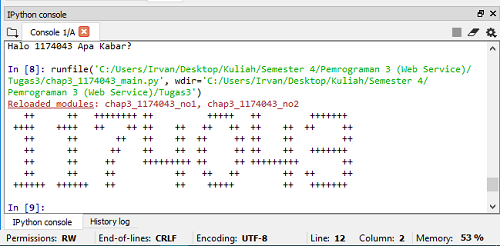
\includegraphics[width=0.6\textwidth]{figures/chapter3/1_1174043.png}}
					\caption{Jawaban No. 1}
					\label{1}
				\end{figure}

				\ref{1_1174043}
				
			\item Jawaban soal no 2
				\lstinputlisting{src/chapter3/chap3_1174043_no2.py}
				
				\begin{figure} [ht]
					\centerline{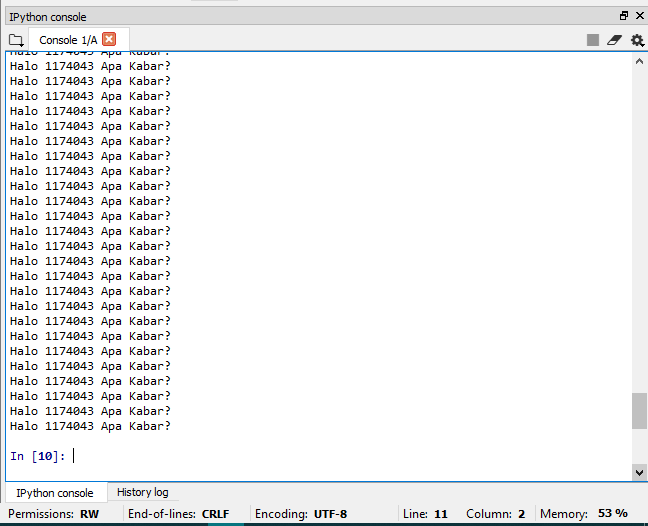
\includegraphics[width=1\textwidth]{figures/chapter3/2_1174043.png}}
					\caption{Jawaban No. 2}
					\label{2}
				\end{figure}

				\ref{2_1174043}
			
			\item Jawaban soal no 3
				\lstinputlisting{src/chapter3/chap3_1174043_no3.py}
				
				\begin{figure} [ht]
					\centerline{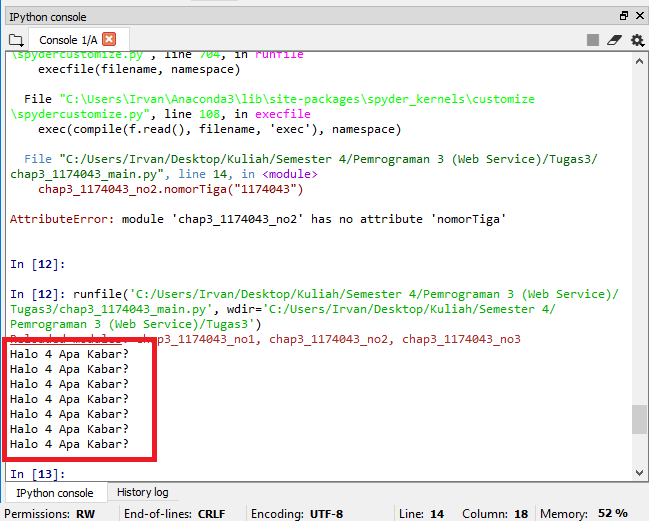
\includegraphics[width=1\textwidth]{figures/chapter3/3_1174043.png}}
					\caption{Jawaban No. 3}
					\label{3}
				\end{figure}

				\ref{3_1174043}
				
			\item Jawaban soal no 4
				\lstinputlisting{src/chapter3/chap3_1174043_no4.py}
				
				\begin{figure} [ht]
					\centerline{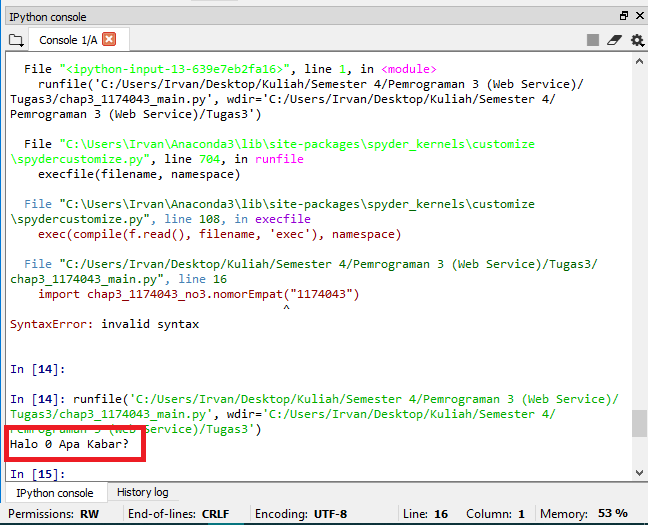
\includegraphics[width=1\textwidth]{figures/chapter3/4_1174043.png}}
					\caption{Jawaban No. 4}
					\label{4}
				\end{figure}

				\ref{4_1174043}
				
			\item Jawaban soal no 5
				\lstinputlisting{src/chapter3/chap3_1174043_no5.py}
				
				\begin{figure} [ht]
					\centerline{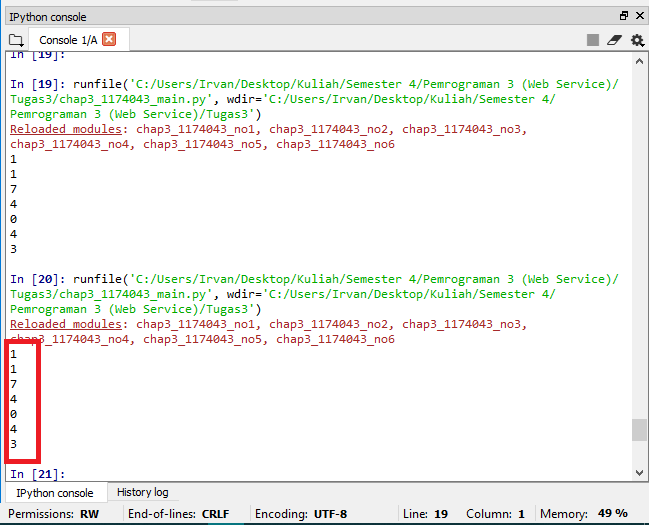
\includegraphics[width=1\textwidth]{figures/chapter3/5_1174043.png}}
					\caption{Jawaban No. 5}
					\label{5}
				\end{figure}

				\ref{5_1174043}
				
			\item Jawaban soal no 6
				\lstinputlisting{src/chapter3/chap3_1174043_no6.py}
				
				\begin{figure} [ht]
					\centerline{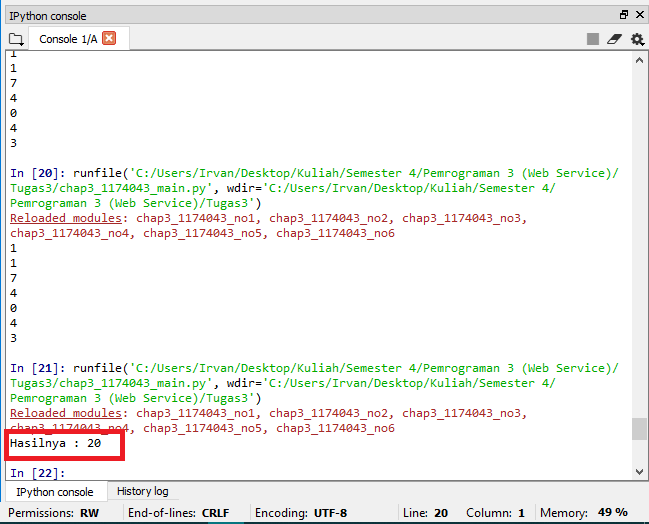
\includegraphics[width=1\textwidth]{figures/chapter3/6_1174043.png}}
					\caption{Jawaban No. 6}
					\label{6}
				\end{figure}

				\ref{6_1174043}
				
			\item Jawaban soal no 7
				\lstinputlisting{src/chapter3/chap3_1174043_no7.py}
				
				\begin{figure} [ht]
					\centerline{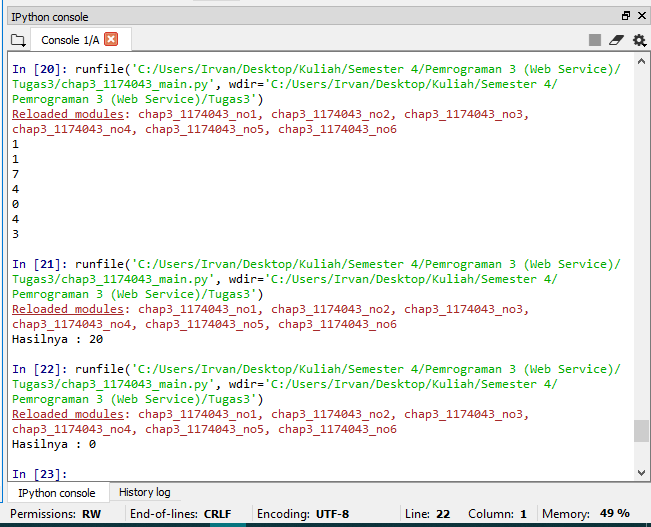
\includegraphics[width=1\textwidth]{figures/chapter3/7_1174043.png}}
					\caption{Jawaban No. 7}
					\label{7}
				\end{figure}

				\ref{7_1174043}
				
			\item Jawaban soal no 8
				\lstinputlisting{src/chapter3/chap3_1174043_no8.py}
				
				\begin{figure} [ht]
					\centerline{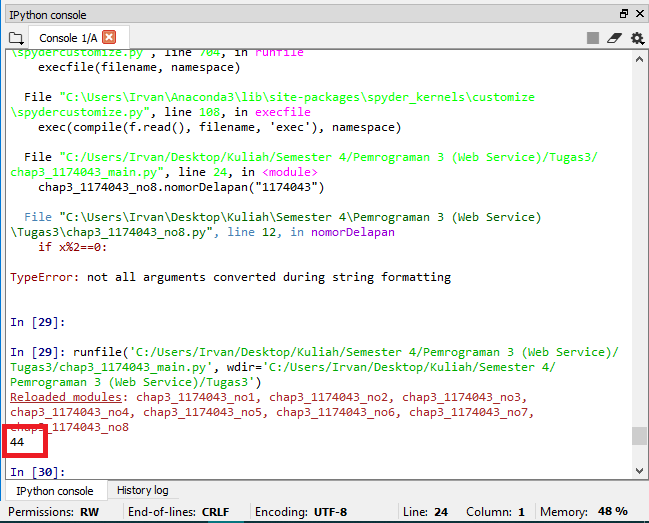
\includegraphics[width=1\textwidth]{figures/chapter3/8_1174043.png}}
					\caption{Jawaban No. 8}
					\label{8}
				\end{figure}

				\ref{8_1174043}
				
			\item Jawaban soal no 9
				\lstinputlisting{src/chapter3/chap3_1174043_no9.py}
				
				\begin{figure} [ht]
					\centerline{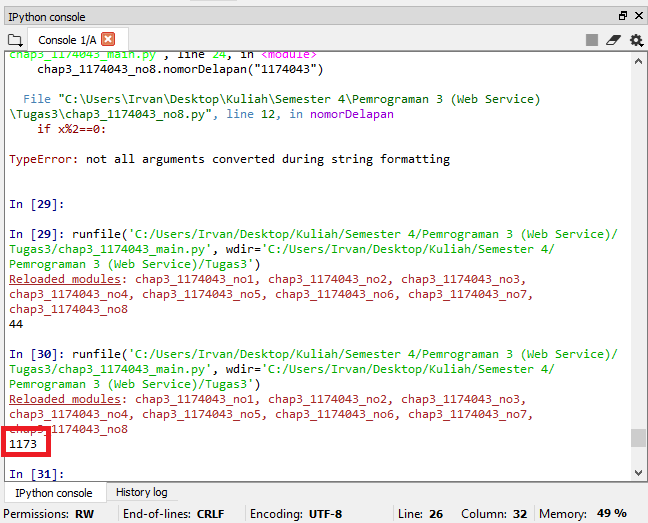
\includegraphics[width=1\textwidth]{figures/chapter3/9_1174043.png}}
					\caption{Jawaban No. 9}
					\label{9}
				\end{figure}

				\ref{9_1174043}
				
			\item Jawaban soal no 10
				\lstinputlisting{src/chapter3/chap3_1174043_no10.py}
				
				\begin{figure} [ht]
					\centerline{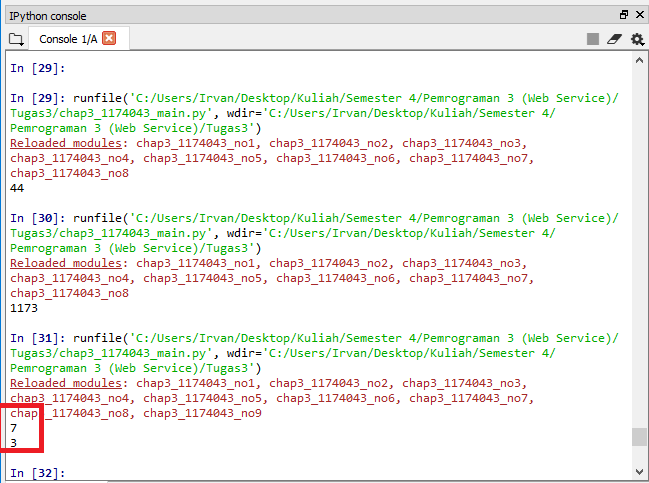
\includegraphics[width=1\textwidth]{figures/chapter3/10_1174043.png}}
					\caption{Jawaban No. 10}
					\label{10}
				\end{figure}

				\ref{10_1174043}
				
			\item Jawaban soal no 11
			
				File 3lib.py
				\lstinputlisting{src/chapter3/chap3_1174043_3lib.py}
				
				File main.py
				\lstinputlisting{src/chapter3/chap3_1174043_main.py}
				
				\begin{figure} [ht]
					\centerline{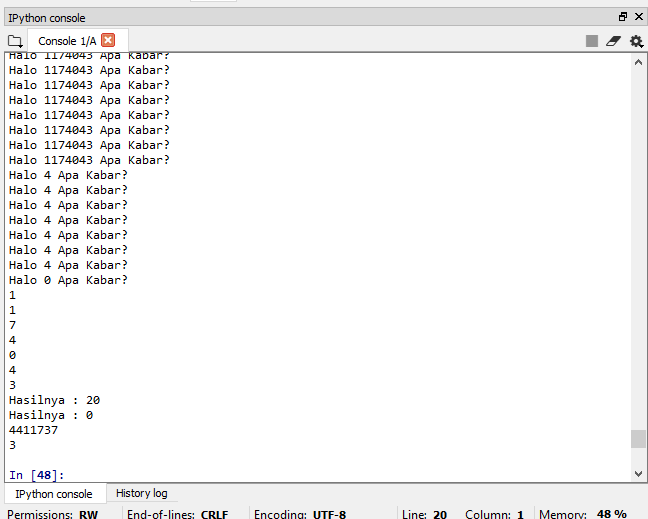
\includegraphics[width=1\textwidth]{figures/chapter3/11_1174043.png}}
					\caption{Jawaban No. 11}
					\label{11}
				\end{figure}

				\ref{11_1174043}
				
			\item Jawaban soal no 12
			\lstinputlisting{src/chapter3/chap3_1174043_kelas3lib.py}
		
		\end{enumerate}
		
		\subsection{Keterampilan Penanganan Error}
			\begin{enumerate}
				\item \lstinputlisting{src/chapter3/chap3_1174043_3err.py}
			
			\end{enumerate}
			
		\subsection{Plagiarisme}
			\begin{figure} [ht]
					\centerline{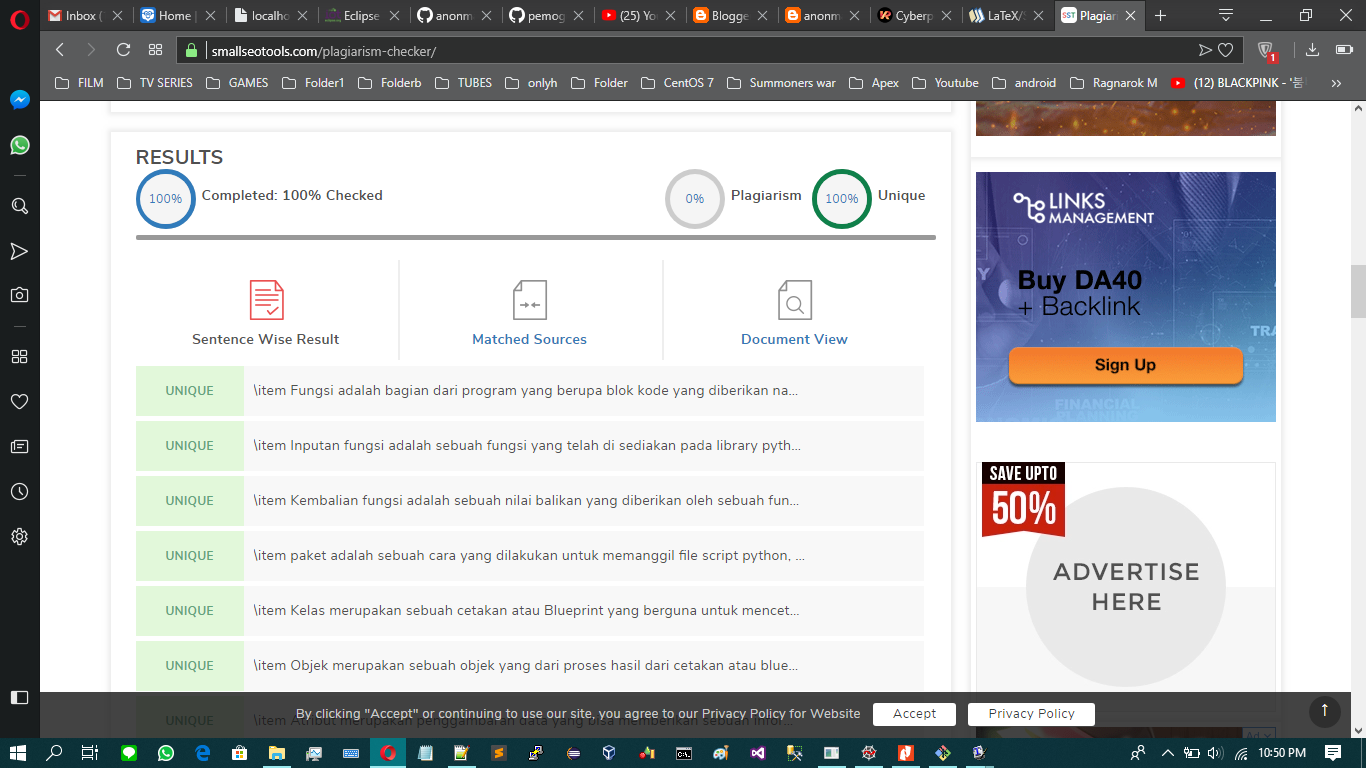
\includegraphics[width=1\textwidth]{figures/chapter3/plagiarisme_1174043.png}}
					\caption{Hasil Cek Plagiarisme}
					\label{plagiarisme}
				\end{figure}

			\ref{plagiarisme_1174043}

\subsection{Luthfi Muhammad Nabil/1174035}
\subsubsection{Pemahaman Teori}
\begin{enumerate}
	\item Fungsi adalah sintaks yang terdiri dari nama fungsi, parameter input variabel, dan variabel kembali. Pada python, nama fungsi diawali dengan def dan pada sintaks paling akhir (setelah parameter) adalah titik dua. Aturan penamaan dari fungsi sama dengan penamaan sebuah variabel yang salah satunya yaitu case sensitive. Untuk penulisan parameter tidak harus memasukan inputan dan batas untuk penulisan variabel pada parameter tidak memiliki batas atau bisa lebih dari satu dengan pemisah tanda koma. Nilai yang dapat dikembalikan oleh fungsi dapat berupa variabel yang mau dikembalikan. Berikut contoh dari koding fungsi : 
	\lstinputlisting[firstline=1, lastline=4]{src/chapter3/chap3_1174035_teori.py}
	\item Paket merupakan sebuah file yang berisikan fungsi - fungsi yang dapat dipakai. Untuk pemanggilan fungsi diperlukan keyword import untuk memanggil paket tersebut. berikut contoh pemakaian dari paket : 
	\lstinputlisting[firstline=6, lastline=8]{src/chapter3/chap3_1174035_teori.py}
	\item Class merupakan cetak biru dari sebuah objek yang dibuat. Objek merupakan instansi dari sebuah class. Atribut merupakan variabel atau yang menampung nilai pada sebuah objek. Fungsi adalah sebuah pembungkus kumpulan instruksi pada sebuah program. Berikut contohnya : 
	\lstinputlisting[firstline=10, lastline=24]{src/chapter3/chap3_1174035_teori.py}
	\item Pemanggilan sebuah kelas diawali dari sebuah paket dipanggil terlebih dahulu, lalu kelas akan disimpan ke variabel untuk diinisiasi sebagai objek. Berikut contoh pemanggilan dari kelas : 
	\lstinputlisting[firstline=26, lastline=29]{src/chapter3/chap3_1174035_teori.py}
	\item Pemakaian from kalkulator merupakan sebuah inisiasi untuk memanggil fungsi penambahan dari paket kalkulator yang dipanggil agar fungsi penambahandapat digunakan langsung tanpa menulis nama file dari paket yaitu kalkulator. Berikut Contohnya : 
	\lstinputlisting[firstline=31, lastline=34]{src/chapter3/chap3_1174035_teori.py}
	\item Pemakaian paket fungsi memanggil fungsi dari paket lain dan memanggil paket tersebut dengan tambahan nama asal paket dari fungsi yang akan dipanggil. Berikut pemakaiannya : 
	\lstinputlisting[firstline=36, lastline=39]{src/chapter3/chap3_1174035_teori.py}
	\item Pemakaian paket kelas sama halnya dengan fungsi hanya saja untuk paket kelas diinisiasikan terlebih dahulu lalu nilai variabel akan dikirim ke constructor dari class tersebut. Pada saat memanggil fungsi tidak perlu menggunakan inputan parameter karena nilai yang dikirim sudah disimpan pada constructor di class yang dipanggil. Berikut Contohnya : 
	\lstinputlisting[firstline=41, lastline=46]{src/chapter3/chap3_1174035_teori.py}
\end{enumerate}
\subsection{Ketrampilan Pemrograman}
\begin{enumerate}
	\item Membuat fungsi dengan inputan variabel NPM, dan melakukan print luaran huruf yang dirangkai dari tanda bintang, paga,r, plus dari NPM kita. Untuk NPM mod 3=0 memakai bintang, NPM mod 3=1 memakai pagar, NPM mod 3 = 2 memakai tanda plus. Kodingnya : 
	\lstinputlisting{src/chapter3/chap3_1174035_1.py}
	\begin{figure}[!htbp]
        \centering
        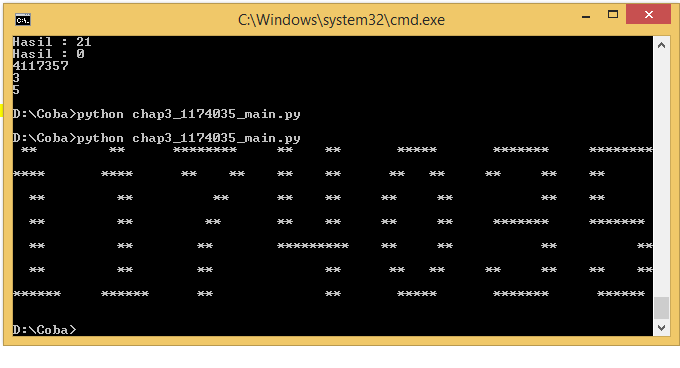
\includegraphics[height=7cm, width=10cm]{figures/chapter3/1174035_1.png}
        \caption{Screenshot No 1}
        \label{1174035_1}
	\end{figure}
	\item Membuat fungsi dengan inputan variabel NPM, dan lakukan perulangan untuk mengeluarkan print output sebanyak dua dijit belakang NPM. Contoh NPM : 1174035 maka akan ada output sebanyak 35 kali dengan tulisan 'Hallo, 1174035 apa kabar?' Kodingnya : 
	\lstinputlisting{src/chapter3/chap3_1174035_2.py}
	\begin{figure}[!htbp]
        \centering
        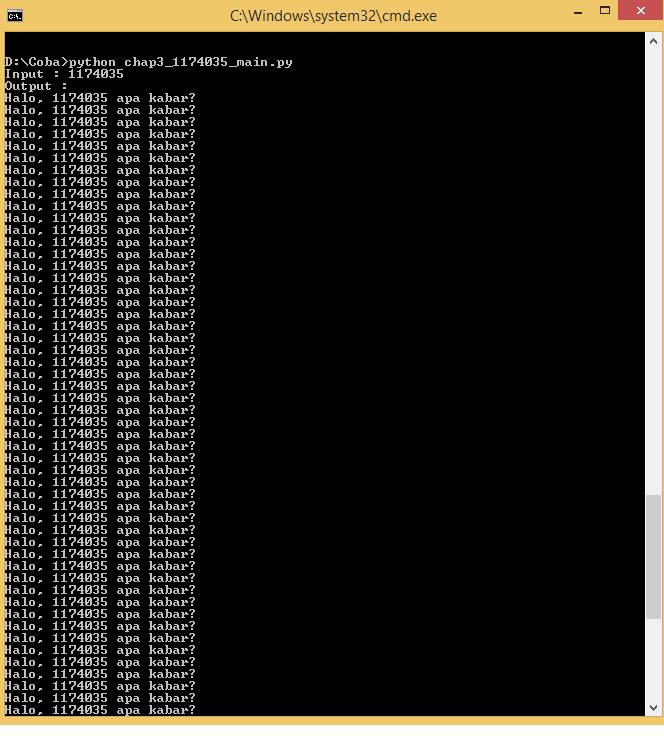
\includegraphics[height=7cm, width=10cm]{figures/chapter3/1174035_2.png}
        \caption{Screenshot No 2}
        \label{1174035_2}
	\end{figure}
	\item Membuat fungsi dengan inputan variabel NPM, dan melakukan print luaran output dengan perulangan berupa tiga karakter belakang dari NPM dijumlahkan. Lalu jumah perulangan tersebut adalah total dari tiga karakter belakang NPM dijumlahkan. Kodingnya : 
	\lstinputlisting{src/chapter3/chap3_1174035_3.py}
	\begin{figure}[!htbp]
        \centering
        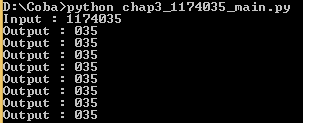
\includegraphics[height=7cm, width=10cm]{figures/chapter3/1174035_3.png}
        \caption{Screenshot No 3}
        \label{1174035_3}
	\end{figure}
	\item Membuat fungsi dengan inputan variabel NPM, dan melakukan print hello world dan digit ketiga dari belakang dari NPM. contoh : NPM : 0, Output : Halo, 0 apa kabar? .Kodingnya : 
	\lstinputlisting{src/chapter3/chap3_1174035_4.py}
	\begin{figure}[!htbp]
        \centering
        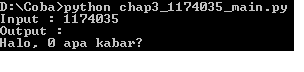
\includegraphics[height=3cm, width=8cm]{figures/chapter3/1174035_4.png}
        \caption{Screenshot No 4}
        \label{1174035_4}
	\end{figure}
	\item Membuat fungsi dengan inputan variabel NPM, dan menampilkan semua angka dari NPM tersebut secara berurutan kebawah. Kodingnya : 
	\lstinputlisting{src/chapter3/chap3_1174035_5.py}
	\begin{figure}[!htbp]
        \centering
        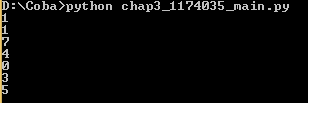
\includegraphics[height=5cm, width=10cm]{figures/chapter3/1174035_5.png}
        \caption{Screenshot No 5}
        \label{1174035_5}
	\end{figure}
	\item Membuat fungsi dengan inputan variabel NPM, didalamnya melakukan penjumlahan dari seluruh dijit NPM tersebut. menggunakan perulangan atau kondisi. Kodingnya : 
	\lstinputlisting{src/chapter3/chap3_1174035_6.py}
	\begin{figure}[!htbp]
        \centering
        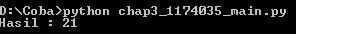
\includegraphics[height=5cm, width=10cm]{figures/chapter3/1174035_6.png}
        \caption{Screenshot No 6}
        \label{1174035_6}
	\end{figure}
	\item Membuat fungsi dengan inputan variabel NPM, didalamnya melakukan perkalian dari seluruh dijit NPM tersebut. menggunakan perulangan atau kondisi. Kodingnya : 
	\lstinputlisting{src/chapter3/chap3_1174035_7.py}
	\begin{figure}[!htbp]
        \centering
        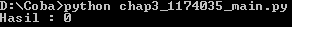
\includegraphics[height=4cm, width=10cm]{figures/chapter3/1174035_7.png}
        \caption{Screenshot No 7}
        \label{1174035_7}
	\end{figure}
	\item Membuat fungsi dengan inputan variabel NPM, lalu lakukan print seluruh angka genap dari setiap angka di NPM. Kodingnya : 
	\lstinputlisting{src/chapter3/chap3_1174035_8.py}
	\begin{figure}[!htbp]
        \centering
        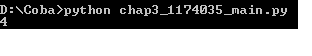
\includegraphics[height=4cm, width=10cm]{figures/chapter3/1174035_8.png}
        \caption{Screenshot No 8}
        \label{1174035_8}
	\end{figure}
	\item Membuat fungsi dengan inputan variabel NPM, lalu lakukan print seluruh angka ganjil dari setiap angka di NPM. Kodingnya : 
	\lstinputlisting{src/chapter3/chap3_1174035_9.py}
	\begin{figure}[!htbp]
        \centering
        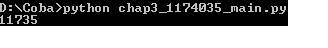
\includegraphics[height=4cm, width=10cm]{figures/chapter3/1174035_9.png}
        \caption{Screenshot No 9}
        \label{1174035_9}
	\end{figure}
	\item Membuat fungsi dengan inputan variabel NPM, lalu lakukan print seluruh angka prima dari setiap angka di NPM. Kodingnya : 
	\lstinputlisting{src/chapter3/chap3_1174035_10.py}
	\begin{figure}[!htbp]
        \centering
        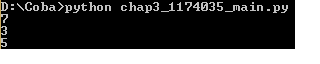
\includegraphics[height=5cm, width=10cm]{figures/chapter3/1174035_10.png}
        \caption{Screenshot No 10}
        \label{1174035_10}
	\end{figure}
	\item Membuat Satu File library bernama 3lib.py yang berisi semua fungsi - fungsi dari setiap nomor pada soal praktek. Kodingnya : 	
	\lstinputlisting{src/chapter3/chap3_1174035_3lib.py}
	\lstinputlisting[firstline=1, lastline=15]{src/chapter3/chap3_1174035_main.py}
	
	\begin{figure}[!htbp]
        \centering
        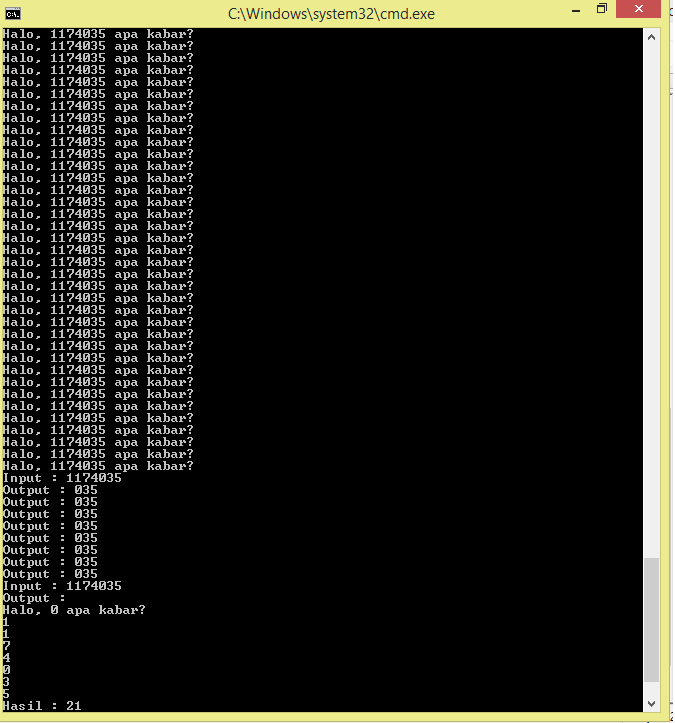
\includegraphics[height=10cm, width=8cm]{figures/chapter3/1174035_3lib.png}
        \caption{Screenshot No 11}
        \label{1174035_3lib}
	\end{figure}
	
	\item Membuat Satu File library bernama kelas3lib.py yang berisi kelas yang isinya semua fungsi - fungsi dari setiap nomor yang telah dimodifikasi untuk menyesuaikan dengan kelas. Kodingnya : 	
	\lstinputlisting{src/chapter3/chap3_1174035_kelas3lib.py}
	\lstinputlisting[firstline=16, lastline=29]{src/chapter3/chap3_1174035_main.py}
	
	\begin{figure}[!htbp]
        \centering
        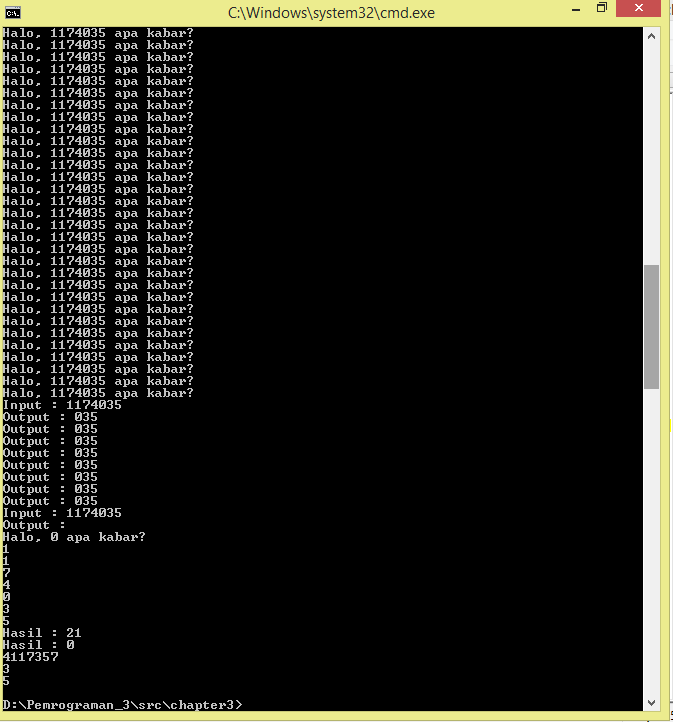
\includegraphics[height=10cm, width=8cm]{figures/chapter3/1174035_kelas3lib.png}
        \caption{Screenshot No 12}
        \label{1174035_kelas3lib}
	\end{figure}
	
	
\end{enumerate}

\subsubsection{Error}
\begin{enumerate}
	\item Tuliskan error yang terjadi saat mengerjakan section ini. Mendapat error yaitu salah konversi. Untuk menghandle error tersebut dapat menggunakan try catch :
	\lstinputlisting{src/chapter3/chap3_1174035_error.py}
	\lstinputlisting[firstline=32, lastline=36]{src/chapter3/chap3_1174035_main.py}
	\begin{figure}[!htbp]
        \centering
        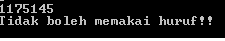
\includegraphics[height=3cm, width=8cm]{figures/chapter3/1174035_error.png}
        \caption{Screenshot No 13}
        \label{1174035_error}
	\end{figure}
	\item Plagiarisme
	\begin{figure}[!htbp]
        \centering
        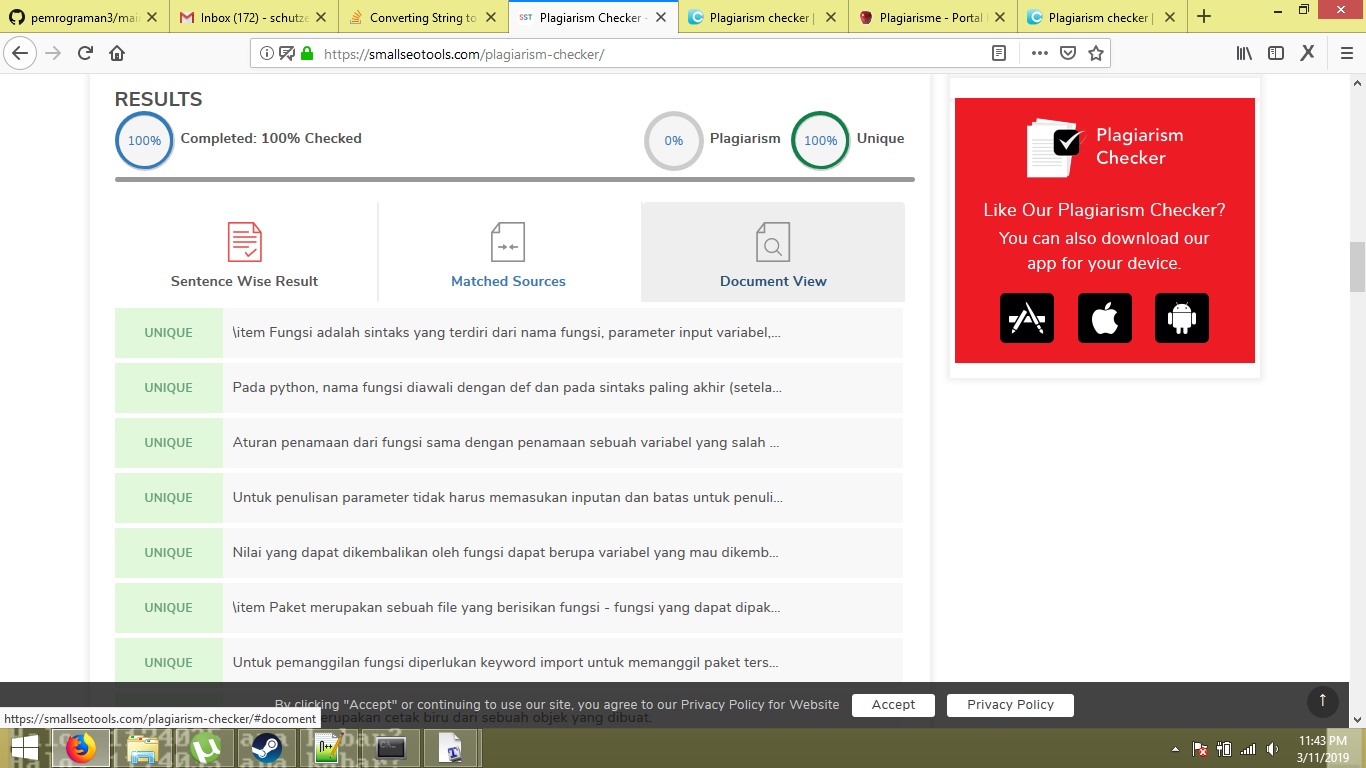
\includegraphics[height=7cm, width=9cm]{figures/chapter3/1174035_plagiarisme.png}
        \caption{Plagiarisme}
        \label{1174035_plagiarisme}
	\end{figure}
\end{enumerate}

\section{Rangga Putra Ramdhani}
\subsubsection{Pemahanan Teori}
\begin{enumerate}
    \item Apa itu fungsi, inputan fungsi dan kembalian fungsi dengan contoh kode program
    lainnya.
    Fungsi adalah bagian dari program yang dapat digunakan ulang.
    Berikut merupakan contoh fungsi dan cara pemanggilannya
    \lstinputlisting[firstline=124, lastline=127]{src/1174056_praktek.py}

    Fungsi dapat membaca parameter, parameter adalah nilai yang disediakan kepada fungsi, dimana nilai ini akan menentukan output yang akan dihasilkan fungsi.
    \lstinputlisting[firstline=129, lastline=132]{src/1174056_praktek.py}

    Statemen return digunakan untuk keluar dari fungsi. Kita juga dapat menspesifikasikan nilai kembalian.
    \lstinputlisting[firstline=134, lastline=141]{src/1174056_praktek.py}

    \item Apa itu paket dan cara pemanggilan paket atau library dengan contoh kode
    program lainnya.
    Untuk memudahkan dalam pemanggilan fungsi yang di butuhkan, agar dapat dipanggil berulang.
    Cara pemanggilannya
    \lstinputlisting[firstline=143, lastline=144]{src/1174056_praktek.py}

    \item Jelaskan Apa itu kelas, apa itu objek, apa itu atribut, apa itu method dan
    contoh kode program lainnya masing-masing.
    kelas merupakan sebuah blueprint yang mepresentasikan objek.
    objek adalah hasil cetakan dadri sebuah kelas.
    method adalah suatu upaya yang digunakan oleh object.
    \lstinputlisting[firstline=146, lastline=168]{src/1174056_praktek.py}

    \item Jelaskan cara pemanggikan library kelas dari instansiasi dan pemakaiannya den-
    gan contoh program lainnya.
    Cara Pemanggilanya 
    \begin{itemize}
        \item pertama import terlebih dahulu filenya.
        \item kemudian buat variabel untuk menampung datanya
        \item setelah itu panggil nama classnya dan panggil methodnya
        \item Gunakan perintah print untuk menampilkan hasilnya

    \end{itemize}
    \lstinputlisting[firstline=170, lastline=175]{src/1174056_praktek.py}

    \item Jelaskan dengan contoh pemakaian paket dengan perintah from kalkulator im-
    port Penambahan disertai dengan contoh kode lainnya.
    Penggunaan paket from namafile import, itu berfungsi untuk memanggil file dan fungsinya
    \lstinputlisting[firstline=143, lastline=144]{src/1174056_praktek.py}

    \item Jelaskan dengan contoh kodenya, pemakaian paket fungsi apabila le library
    ada di dalam folder.
    Pemakaian paket adalah perkumpulan fungsi-fungsi. contoh kodenya adalah sebagai berikut :

    \item Jelaskan dengan contoh kodenya, pemakaian paket kelas apabila le library ada
    di dalam folder.
    \lstinputlisting[firstline=184, lastline=184]{src/1174056_praktek.py}

\end{enumerate}
\subsubsection{Ketrampilan Pemrograman}
\begin{enumerate}
    \item Buatlah fungsi dengan inputan variabel NPM, dan melakukan print luaran huruf
    yang dirangkai dari tanda bintang, pagar atau plus dari NPM kita. Tanda
    bintang untuk NPM mod 3=0, tanda pagar untuk NPM mod 3 =1, tanda plus
    untuk NPM mod3=2.
    \lstinputlisting[firstline=184, lastline=234]{src/1174056_praktek.py}

    \item Buatlah fungsi dengan inputan variabel berupa NPM. kemudian dengan meng-
    gunakan perulangan mengeluarkan print output sebanyak dua dijit belakang
    NPM.
    \lstinputlisting[firstline=237, lastline=243]{src/1174056_praktek.py}

    \item Buatlah fungsi dengan dengan input variabel string bernama NPM dan beri
    luaran output dengan perulangan berupa tiga karakter belakang dari NPM se-
    banyak penjumlahan tiga dijit tersebut.
    \lstinputlisting[firstline=245, lastline=255]{src/1174056_praktek.py}

    \item Buatlah fungsi hello word dengan input variabel string bernama NPM dan
    beri luaran output berupa digit ketiga dari belakang dari variabel NPM meng-
    gunakan akses langsung manipulasi string pada baris ketiga dari variabel NPM.
    \lstinputlisting[firstline=257, lastline=263]{src/1174056_praktek.py}

    \item buat fungsi program dengan input variabel NPM dan melakukan print nomor npm satu persatu kebawah.
    \lstinputlisting[firstline=265, lastline=269]{src/1174056_praktek.py}

    \item Buatlah fungsi dengan inputan variabel NPM, didalamnya melakukan penjum-
    lahan dari seluruh dijit NPM tersebut, wajib menggunakan perulangan dan
    atau kondisi.
    \lstinputlisting[firstline=272, lastline=279]{src/1174056_praktek.py}

    \item Buatlah fungsi dengan inputan variabel NPM, didalamnya melakukan melakukan
    perkalian dari seluruh dijit NPM tersebut, wajib menggunakan perulangan dan
    atau kondisi.
    \lstinputlisting[firstline=281, lastline=288]{src/1174056_praktek.py}

    \item Buatlah fungsi dengan inputan variabel NPM, Lakukan print NPM anda tapi
    hanya dijit genap saja. wajib menggunakan perulangan dan atau kondisi.
    \lstinputlisting[firstline=290, lastline=296]{src/1174056_praktek.py}

    \item Buatlah fungsi dengan inputan variabel NPM, Lakukan print NPM anda tapi
    hanya dijit ganjil saja. wajib menggunakan perulangan dan atau kondisi.
    \lstinputlisting[firstline=298, lastline=304]{src/1174056_praktek.py}

    \item Buatlah fungsi dengan inputan variabel NPM, Lakukan print NPM anda tapi
    hanya dijit yang termasuk bilangan prima saja. wajib menggunakan perulangan
    dan atau kondisi.
    \lstinputlisting[firstline=306, lastline=320]{src/1174056_praktek.py}

    \item Buatlah satu library yang berisi fungsi-fungsi dari nomor diatas dengan nama
    le rangga.py dan berikan contoh cara pemanggilannya pada le main.py.
    \lstinputlisting[firstline=7, lastline=7]{src/mainn.py}

    \item Buatlah satu library class dengan nama le kelas3lib.py yang merupakan mod-
    ikasi dari fungsi-fungsi nomor diatas dan berikan contoh cara pemanggilannya
    pada le mainn.py.
    \lstinputlisting[firstline=8, lastline=9]{src/mainn.py}
    
\end{enumerate}
\subsubsection{Ketrampilan Penanganan Error}
Error yang di dapat dari mengerjakan tugas ini adalah type error, cara menaggulaginya dengan cara mengecheck kembali codingannya
kemudian run kembali aplikasinya
berikut contoh Penggunaan fungsi try dan exception
\lstinputlisting[firstline=177, lastline=182]{src/1174056_praktek.py}


\section{Faisal Najib Abdullah}
\subsection{Pemahanan Teori}
\begin{enumerate}
    \item Apa itu fungsi, inputan fungsi dan kembalian fungsi dengan contoh kode program
    lainnya.
    Fungsi adalah bagian dari program yang dapat digunakan ulang.
    Berikut merupakan contoh fungsi dan cara pemanggilannya
    \lstinputlisting{src/chapter3/1174042_1,1.py}

    Fungsi dapat membaca parameter, parameter adalah nilai yang disediakan kepada fungsi, dimana nilai ini akan menentukan output yang akan dihasilkan fungsi.
    \lstinputlisting{src/chapter3/1174042_1,1,1.py}

    Statemen return digunakan untuk keluar dari fungsi. Kita juga dapat menspesifikasikan nilai kembalian.
    \lstinputlisting{src/chapter3/1174042_1,1,2.py}

    \item Apa itu paket dan cara pemanggilan paket atau library dengan contoh kode
    program lainnya.
    Untuk memudahkan dalam pemanggilan fungsi yang di butuhkan, agar dapat dipanggil berulang.
    Cara pemanggilannya
    \lstinputlisting{src/chapter3/1174042_1,2.py}

    \item Jelaskan Apa itu kelas, apa itu objek, apa itu atribut, apa itu method dan
    contoh kode program lainnya masing-masing.
    kelas merupakan sebuah blueprint yang mepresentasikan objek.
    objek adalah hasil cetakan dadri sebuah kelas.
    method adalah suatu upaya yang digunakan oleh object.
    \lstinputlisting{src/chapter3/1174042_1,3.py}

    \item Jelaskan cara pemanggikan library kelas dari instansiasi dan pemakaiannya den-
    gan contoh program lainnya.
    Cara Pemanggilanya 
    \begin{itemize}
        \item pertama import terlebih dahulu filenya.
        \item kemudian buat variabel untuk menampung datanya
        \item setelah itu panggil nama classnya dan panggil methodnya
        \item Gunakan perintah print untuk menampilkan hasilnya

    \end{itemize}
    \lstinputlisting{src/chapter3/1174042_1,4.py}

    \item Jelaskan dengan contoh pemakaian paket dengan perintah from kalkulator im-
    port Penambahan disertai dengan contoh kode lainnya.
    Penggunaan paket from namafile import, itu berfungsi untuk memanggil file dan fungsinya
    \lstinputlisting{src/chapter3/1174042_1,2.py}

    \item Jelaskan dengan contoh kodenya, pemakaian paket fungsi apabila file library
    ada di dalam folder.
    Pemakaian paket adalah perkumpulan fungsi-fungsi. contoh kodenya adalah sebagai berikut :
	\lstinputlisting{src/chapter3/1174042_1,6.py}

    \item Jelaskan dengan contoh kodenya, pemakaian paket kelas apabila file library ada
    di dalam folder.
    \lstinputlisting{src/chapter3/1174042_1,6.py}

	\end{enumerate}

\subsection{Ketrampilan Pemrograman}
\begin{enumerate}
    \item Buatlah fungsi dengan inputan variabel NPM, dan melakukan print luaran huruf
    yang dirangkai dari tanda bintang, pagar atau plus dari NPM kita. Tanda
    bintang untuk NPM mod 3=0, tanda pagar untuk NPM mod 3 =1, tanda plus
    untuk NPM mod3=2.
    \lstinputlisting{src/chapter3/1174042_2,1.py}

    \item Buatlah fungsi dengan inputan variabel berupa NPM. kemudian dengan meng-
    gunakan perulangan mengeluarkan print output sebanyak dua dijit belakang
    NPM.
    \lstinputlisting{src/chapter3/1174042_2,2.py}

    \item Buatlah fungsi dengan dengan input variabel string bernama NPM dan beri
    luaran output dengan perulangan berupa tiga karakter belakang dari NPM se-
    banyak penjumlahan tiga dijit tersebut.
    \lstinputlisting{src/chapter3/1174042_2,3.py}

    \item Buatlah fungsi hello word dengan input variabel string bernama NPM dan
    beri luaran output berupa digit ketiga dari belakang dari variabel NPM meng-
    gunakan akses langsung manipulasi string pada baris ketiga dari variabel NPM.
    \lstinputlisting{src/chapter3/1174042_2,4.py}

    \item buat fungsi program dengan input variabel NPM dan melakukan print nomor npm satu persatu kebawah.
    \lstinputlisting{src/chapter3/1174042_2,5.py}

    \item Buatlah fungsi dengan inputan variabel NPM, didalamnya melakukan penjum-
    lahan dari seluruh dijit NPM tersebut, wajib menggunakan perulangan dan
    atau kondisi.
    \lstinputlisting{src/chapter3/1174042_2,6.py}

    \item Buatlah fungsi dengan inputan variabel NPM, didalamnya melakukan melakukan
    perkalian dari seluruh dijit NPM tersebut, wajib menggunakan perulangan dan
    atau kondisi.
    \lstinputlisting{src/chapter3/1174042_2,7.py}

    \item Buatlah fungsi dengan inputan variabel NPM, Lakukan print NPM anda tapi
    hanya dijit genap saja. wajib menggunakan perulangan dan atau kondisi.
    \lstinputlisting{src/chapter3/1174042_2,8.py}

    \item Buatlah fungsi dengan inputan variabel NPM, Lakukan print NPM anda tapi
    hanya dijit ganjil saja. wajib menggunakan perulangan dan atau kondisi.
    \lstinputlisting{src/chapter3/1174042_2,9.py}

    \item Buatlah fungsi dengan inputan variabel NPM, Lakukan print NPM anda tapi
    hanya dijit yang termasuk bilangan prima saja. wajib menggunakan perulangan
    dan atau kondisi.
    \lstinputlisting{src/chapter3/1174042_2,10.py}

    \item Buatlah satu library yang berisi fungsi-fungsi dari nomor diatas dengan nama
    file 3lib.py dan berikan contoh cara pemanggilannya pada file main.py.
    \lstinputlisting{src/chapter3/1174042_main.py}

    \item Buatlah satu library class dengan nama file kelas3lib.py yang merupakan mod-
    ifikasi dari fungsi-fungsi nomor diatas dan berikan contoh cara pemanggilannya
    pada file main.py.
    \lstinputlisting{src/chapter3/1174042_main.py}
    
\end{enumerate}
\subsection{Ketrampilan Penanganan Error}
Error yang di dapat dari mengerjakan tugas ini adalah type error, cara menaggulaginya dengan cara mengecheck kembali codingannya
kemudian run kembali aplikasinya
berikut contoh Penggunaan fungsi try dan exception
\lstinputlisting{src/chapter3/1174042_2err.py}

\section{Yusniar Nur Syarif Sidiq/1164089}
\subsection{Teori}
\begin{enumerate}
\item Fungsi merupakan sebuah bagian dari program yang dapat digunakan ulang dan memiliki inputan variabel serta nilai yang akan di kembalikannya. Contohnya adalah source code berikut ini,
	 \lstinputlisting{src/chapter2/1164089/1164089_1.py}
Dalam dalam source code tersebut akan mengeluarkan output Hallo 1164089 ketika kita running di dalam spyder.

\item Library dalam python disini merupakan kumpulan dari fungsi dan cara pemanggilannya adalah dengan melakukan import file librarynya. Sebagai contoh, buatlah Matematika.py dan 1164089\_2.py, simpan dalam satu folder. Untuk Matematika.py isikan fungsi sebagai berikut
	 \lstinputlisting{src/chapter2/1164089/Matematika.py}
Untuk memanggil fungsi tersebut adalah dengan melakukan import  Matematika.py pada 1164089\_2.py adalah sebagai berikut,
	 \lstinputlisting{src/chapter2/1164089/1164089_2.py}

\item Class merupakan salah satu cara untuk membuat sebuah kode yang mempunyai objek serta atribut tertentu sehingga akan lebih mudah dalam mengorganisasi berbagai fungsi dan statenya. Objek disini merupakan instansiasi atau perwujudan dari sebuah class. Untuk membuat class yang memiliki objek serta atribut dapat dilihat pada source code berikut ini, dimana kita akan membaut file bernama mtk.py
	\lstinputlisting{src/chapter2/1164089/mtk.py}
Self tersebut berfungsi untuk menunjukkan variabel lokal dari class tersebut. Untuk memanggil class tersebut kita akan membuat file bernama 1164089\_3.py dan kita akan melakukan import mtk.py pada file tersebut, untuk source codenya dapat dilihat seperti berikut,
	\lstinputlisting{src/chapter2/1164089/1164089_3.py}

\item Cara memanggilnya yaitu
	\begin{itemize}
		\item Pertama import terlebih dahulu filenya
		\item Buat variabel yang berfungsi menampung data
		\item Panggil nama classnya dan methodnya
		\item Gunakan perintah print untuk menampilkannya
	\end{itemize}
Sebagai contoh perhatikan source code ini,
	\lstinputlisting{src/chapter2/1164089/1164089_4.py}

\item Dimana kita akan melakukan membuka library Matematika.py dan akan melakukan import dari fungsi di dalamnya yaitu matematika, sehingga akan lebih simple dalam penulisan source codenya adalah sebagai berikut,
	\lstinputlisting{src/chapter2/1164089/1164089_5.py}

\item

\item 
\end{enumerate}

\subsection{Keterampilan Pemrograman}
\begin{enumerate}

\item Soal No 1 \lstinputlisting{src/chapter2/1164089/1164089_21.py}

\item Soal No 2 \lstinputlisting{src/chapter2/1164089/1164089_22.py}

\item Soal No 3 \lstinputlisting{src/chapter2/1164089/1164089_23.py}

\item Soal No 4 \lstinputlisting{src/chapter2/1164089/1164089_24.py}

\item Soal No 5 \lstinputlisting{src/chapter2/1164089/1164089_25.py}

\item Soal No 6 \lstinputlisting{src/chapter2/1164089/1164089_26.py}

\item Soal No 7 \lstinputlisting{src/chapter2/1164089/1164089_27.py}

\item Soal No 8 \lstinputlisting{src/chapter2/1164089/1164089_28.py}

\item Soal No 9 \lstinputlisting{src/chapter2/1164089/1164089_29.py}

\item Soal No 10 \lstinputlisting{src/chapter2/1164089/1164089_30.py}

\item Soal No 11 \lstinputlisting{src/chapter2/1164089/1164089_31.py}

\item Soal No 12 \lstinputlisting{src/chapter2/1164089/1164089_32.py}
\end{enumerate}

\subsection{Penanganan Erorr}
\begin{enumerate}

\item Erorr yang saya temui di antaranya adalah Systax Erorr, dimana suatu keadaan script python mengalami kesalahan dalam penulisannya dan solusi dari permasalahan ini adalah dengan memperbaiki script penulisan yang salah. Untuk contoh fungsi trx except dapat dilihat pada source code berikut ini,

	\lstinputlisting{src/chapter2/1164089/1164089_33.py}

\end{enumerate}

\section{Fathi Rabbani/1164074/3C}
\subsection{Teori}
\begin{enumerate}
\item Fungsi, Inputan dan Return
	\begin{itemize}
	\item Fungsi adalah sebuah blok code yang digunakan untuk melempar parameter kedalam blok code yang berbeda.
		\lstinputlisting[firstline=9, lastline=11]{src/chapter3/1164074/praktek.py}
	\item Inputan fungsi adalah sebuah fungsi yang memiliki parameter berupa inputan atau data yang bias diinputkan.
		\lstinputlisting[firstline=13, lastline=15]{src/chapter3/1164074/praktek.py}
	\item Pengembalian fungsi atau sering juga disebut sebagai return merupakan sebuah pengembalian nilai dari pengeksekusian data pada parameter yang terdapat difungsi.
		\lstinputlisting[firstline=17, lastline=24]{src/chapter3/1164074/praktek.py}
	\end{itemize}

\item Paket atau Library Fungsi
	\subitem paket merupakan sebuah penggunaan library dengan maksud mempermudah dalam eksekusi dan pemanggilan fungsi
		\lstinputlisting[firstline=171, lastline=173]{src/chapter3/1164074/praktek.py}
	berikut ini adalah fungsi yang digunakan untuk memanggil paket atau library
		\lstinputlisting[firstline=175, lastline=178]{src/chapter3/1164074/praktek.py}
\item Kelas, Objek, Atribut dan Method
	\begin{itemize}
	\item kelas merupakan sebuah blueprint dari objek
	\item objek merupakan sebuah data hasil eksekusi dari kelas
	\item atribut merupakan nilai data yang terdapat didalam objek
	\item method merupakan operasi atau eksekusi yang dilakukan dengan data dari objek
		\lstinputlisting[firstline=1, lastline=7]{src/chapter3/1164074/praktek.py}
	\end{itemize}
\item Library Kelas
	\begin{itemize}
	\item Penggunaan kelas dan datanya
		\lstinputlisting[firstline=1, lastline=7]{src/chapter3/1164074/praktek.py}
	\item Pemanggilan library kelas
		\lstinputlisting[firstline=181, lastline=186]{src/chapter3/1164074/praktek.py}
	\end{itemize}
\item Pemanggilan Library Kalkulator
	\begin{itemize}
	\item data Kalkulator
		\lstinputlisting[firstline=189, lastline=191]{src/chapter3/1164074/praktek.py}
	\item data pemanggilan
		\lstinputlisting[firstline=193, lastline=198]{src/chapter3/1164074/praktek.py}
	\end{itemize}
\item Penggunaan Paket Fungsi
	\begin{itemize}
	\item data Fungsi Kalkulator
		\lstinputlisting[firstline=189, lastline=191]{src/chapter3/1164074/praktek.py}
	\item data Pemanggil Fungsi
		\lstinputlisting[firstline=200, lastline=203]{src/chapter3/1164074/praktek.py}
	\end{itemize}
\item Penggunaan Paket Kelas
	\begin{itemize}
	\item data Kelas fthr dari file praktek
		\lstinputlisting[firstline=1, lastline=7]{src/chapter3/1164074/praktek.py}
	\item data pemanggil
		\lstinputlisting[firstline=183, lastline=188]{src/chapter3/1164074/praktek.py}
	\end{itemize}
\end{enumerate}

\subsection{Praktek Pemrograman}
	\begin{enumerate}
	\item\lstinputlisting[firstline=27, lastline=74]{src/chapter3/1164074/praktek.py}
	\item\lstinputlisting[firstline=77, lastline=82]{src/chapter3/1164074/praktek.py}
	\item\lstinputlisting[firstline=85, lastline=96]{src/chapter3/1164074/praktek.py}
	\item\lstinputlisting[firstline=99, lastline=103]{src/chapter3/1164074/praktek.py}
	\item\lstinputlisting[firstline=106, lastline=110]{src/chapter3/1164074/praktek.py}
	\item\lstinputlisting[firstline=113, lastline=119]{src/chapter3/1164074/praktek.py}
	\item\lstinputlisting[firstline=122, lastline=128]{src/chapter3/1164074/praktek.py}
	\item\lstinputlisting[firstline=131, lastline=138]{src/chapter3/1164074/praktek.py}
	\item\lstinputlisting[firstline=141, lastline=147]{src/chapter3/1164074/praktek.py}
	\item\lstinputlisting[firstline=150, lastline=158]{src/chapter3/1164074/praktek.py}
	\item
		\begin{itemize}
		\item data 3lib.py
			\lstinputlisting[firstline=17, lastline=191]{src/chapter3/1164074/3lib.py}
		\item data main.py
			\lstinputlisting[firstline=1, lastline=5]{src/chapter3/1164074/main.py}
		\end{itemize}
	\end{enumerate}

\subsection{Handling Error}
\par Error yang di dapat dari mengerjakan tugas ini adalah type error, cara menaggulaginya dengan cara mengecheck kembali codingannya, kemudian run kembali aplikasinya berikut adalah contoh Penggunaan fungsi try dan exception :
\lstinputlisting[firstline=161, lastline=168]{src/chapter3/1164074/praktek.py}



\section{Dika Sukma Pradana 1174050}
\subsection{Pemahanan Teori}
\begin{enumerate}
    \item Apa itu fungsi, inputan fungsi dan kembalian fungsi dengan contoh kode program
    lainnya.
    Fungsi adalah bagian dari program yang dapat digunakan ulang.
    Berikut merupakan contoh fungsi dan cara pemanggilannya
    \lstinputlisting[firstline=124, lastline=127]{src/chapter3/1174050_praktek.py}

    Fungsi dapat membaca parameter, parameter adalah nilai yang disediakan kepada fungsi, dimana nilai ini akan menentukan output yang akan dihasilkan fungsi.
    \lstinputlisting[firstline=129, lastline=132]{src/chapter3/1174050_praktek.py}

    Statemen return digunakan untuk keluar dari fungsi. Kita juga dapat menspesifikasikan nilai kembalian.
    \lstinputlisting[firstline=134, lastline=141]{src/chapter3/1174050_praktek.py}

    \item Apa itu paket dan cara pemanggilan paket atau library dengan contoh kode
    program lainnya.
    Untuk memudahkan dalam pemanggilan fungsi yang di butuhkan, agar dapat dipanggil berulang.
    Cara pemanggilannya
    \lstinputlisting[firstline=143, lastline=144]{src/chapter3/1174050_praktek.py}

    \item Jelaskan Apa itu kelas, apa itu objek, apa itu atribut, apa itu method dan
    contoh kode program lainnya masing-masing.
    kelas merupakan sebuah blueprint yang mepresentasikan objek.
    objek adalah hasil cetakan dadri sebuah kelas.
    method adalah suatu upaya yang digunakan oleh object.
    \lstinputlisting[firstline=146, lastline=168]{src/chapter3/1174050_praktek.py}

    \item Jelaskan cara pemanggikan library kelas dari instansiasi dan pemakaiannya den-
    gan contoh program lainnya.
    Cara Pemanggilanya 
    \begin{itemize}
        \item pertama import terlebih dahulu filenya.
        \item kemudian buat variabel untuk menampung datanya
        \item setelah itu panggil nama classnya dan panggil methodnya
        \item Gunakan perintah print untuk menampilkan hasilnya

    \end{itemize}
    \lstinputlisting[firstline=170, lastline=175]{src/chapter3/1174050_praktek.py}

    \item Jelaskan dengan contoh pemakaian paket dengan perintah from kalkulator im-
    port Penambahan disertai dengan contoh kode lainnya.
    Penggunaan paket from namafile import, itu berfungsi untuk memanggil file dan fungsinya
    \lstinputlisting[firstline=143, lastline=144]{src/chapter3/1174050_praktek.py}

    \item Jelaskan dengan contoh kodenya, pemakaian paket fungsi apabila file library
    ada di dalam folder.
    Pemakaian paket adalah perkumpulan fungsi-fungsi. contoh kodenya adalah sebagai berikut :

    \item Jelaskan dengan contoh kodenya, pemakaian paket kelas apabila file library ada
    di dalam folder.
    \lstinputlisting[firstline=184, lastline=184]{src/chapter3/1174050_praktek.py}

\end{enumerate}
\subsection{Ketrampilan Pemrograman}
\begin{enumerate}
    \item Buatlah fungsi dengan inputan variabel NPM, dan melakukan print luaran huruf
    yang dirangkai dari tanda bintang, pagar atau plus dari NPM kita. Tanda
    bintang untuk NPM mod 3=0, tanda pagar untuk NPM mod 3 =1, tanda plus
    untuk NPM mod3=2.
    \lstinputlisting[firstline=184, lastline=234]{src/chapter3/1174050_praktek.py}

    \item Buatlah fungsi dengan inputan variabel berupa NPM. kemudian dengan meng-
    gunakan perulangan mengeluarkan print output sebanyak dua dijit belakang
    NPM.
    \lstinputlisting[firstline=237, lastline=243]{src/chapter3/1174050_praktek.py}

    \item Buatlah fungsi dengan dengan input variabel string bernama NPM dan beri
    luaran output dengan perulangan berupa tiga karakter belakang dari NPM se-
    banyak penjumlahan tiga dijit tersebut.
    \lstinputlisting[firstline=245, lastline=255]{src/chapter3/1174050_praktek.py}

    \item Buatlah fungsi hello word dengan input variabel string bernama NPM dan
    beri luaran output berupa digit ketiga dari belakang dari variabel NPM meng-
    gunakan akses langsung manipulasi string pada baris ketiga dari variabel NPM.
    \lstinputlisting[firstline=257, lastline=263]{src/chapter3/1174050_praktek.py}

    \item buat fungsi program dengan input variabel NPM dan melakukan print nomor npm satu persatu kebawah.
    \lstinputlisting[firstline=265, lastline=269]{src/chapter3/1174050_praktek.py}

    \item Buatlah fungsi dengan inputan variabel NPM, didalamnya melakukan penjum-
    lahan dari seluruh dijit NPM tersebut, wajib menggunakan perulangan dan
    atau kondisi.
    \lstinputlisting[firstline=272, lastline=279]{src/chapter3/1174050_praktek.py}

    \item Buatlah fungsi dengan inputan variabel NPM, didalamnya melakukan melakukan
    perkalian dari seluruh dijit NPM tersebut, wajib menggunakan perulangan dan
    atau kondisi.
    \lstinputlisting[firstline=281, lastline=288]{src/chapter3/1174050_praktek.py}

    \item Buatlah fungsi dengan inputan variabel NPM, Lakukan print NPM anda tapi
    hanya dijit genap saja. wajib menggunakan perulangan dan atau kondisi.
    \lstinputlisting[firstline=290, lastline=296]{src/chapter3/1174050_praktek.py}

    \item Buatlah fungsi dengan inputan variabel NPM, Lakukan print NPM anda tapi
    hanya dijit ganjil saja. wajib menggunakan perulangan dan atau kondisi.
    \lstinputlisting[firstline=298, lastline=304]{src/chapter3/1174050_praktek.py}

    \item Buatlah fungsi dengan inputan variabel NPM, Lakukan print NPM anda tapi
    hanya dijit yang termasuk bilangan prima saja. wajib menggunakan perulangan
    dan atau kondisi.
    \lstinputlisting[firstline=306, lastline=320]{src/chapter3/1174050_praktek.py}

    \item Buatlah satu library yang berisi fungsi-fungsi dari nomor diatas dengan nama
    file fungsi\_d1ka\_1174050.py dan berikan contoh cara pemanggilannya pada file 1174050\_maiiinn.py.
    \lstinputlisting[firstline=7, lastline=7]{src/chapter3/1174050_maiiinn.py}

    \item Buatlah satu library class dengan nama file kelas3lib\_1174050.py yang merupakan mod-
    ifikasi dari fungsi-fungsi nomor diatas dan berikan contoh cara pemanggilannya      
    pada file 1174050\_maiiinn.py.
    \lstinputlisting[firstline=1, lastline=9]{src/chapter3/1174050_errord1ka.py}
    
\end{enumerate}
\subsection{Ketrampilan Penanganan Error}
Error yang di dapat dari mengerjakan tugas ini adalah type error, cara menaggulaginya dengan cara mengecheck kembali codingannya
kemudian run kembali aplikasinya
berikut contoh Penggunaan fungsi try dan exception
\lstinputlisting[firstline=1, lastline=9]{src/chapter3/1174050_errord1ka.py}


\section{Mhd Zulfikar Akram Nasution/1164081}
\subsection{Teori}
\begin{enumerate}
\item Fungsi merupakan sebuah bagian dari program yang dapat digunakan ulang dan memiliki inputan variable serta nilai yang akan di kembalikan. Contohnya adalah source code berikut ini,
	 \lstinputlisting{src/chapter3/1164081/1164081_1.py}
Dalam dalam source code tersebut akan mengeluarkan output Namaste 1164081 ketika kita running di dalam spyder.

\item Library dalam pythoni merupakan kumpulan dari fungsi, cara pemanggilannya adalah dengan melakukan import file librarynya. Sebagai contoh, buatlah Matematika.py dan 1164081\_2.py, simpan dalam satu folder. Untuk Matematika.py isikan fungsi sebagai berikut
	 \lstinputlisting{src/chapter3/1164081/Matematika.py}
Untuk memanggil fungsi tersebut adalah dengan melakukan import  Matematika.py pada 1164081\_2.py adalah sebagai berikut,
	 \lstinputlisting{src/chapter3/1164081/1164081_2.py}

\item Class merupakan salah satu cara untuk membuat sebuah kode yang mempunyai objek dan atribut tertentu sehingga akan lebih mudah dalam mengorganisasikan berbagai fungsi dan statenya. Objek disini merupakan instansiasi atau perwujudan dari sebuah class. Untuk membuat class yang memiliki objek dan atribut dapat dilihat pada source code berikut ini, dimana kita akan membaut file bernama contoh.py
	\lstinputlisting{src/chapter3/1164081/contoh.py}
Self tersebut berfungsi untuk menunjukkan variabel lokal dari class tersebut. Untuk memanggil class tersebut kita akan membuat file bernama 1164081\_3.py dan kita akan melakukan import contoh.py pada file tersebut, untuk source codenya dapat dilihat seperti berikut,
	\lstinputlisting{src/chapter3/1164081/1164081_3.py}

\item Cara memanggilnya yaitu
	\begin{itemize}
		\item Pertama import terlebih dahulu filenya
		\item Kemudian buat variabel yang berfungsi untuk menampung data
		\item Lalu panggil nama class dan methodnya
		\item Setelah memanggil class dan methodnya, gunakan perintah print untuk menampilkannya
	\end{itemize}
Sebagai contoh perhatikan source code ini,
	\lstinputlisting{src/chapter3/1164081/1164081_4.py}

\item  Penggunaan paket from namafile import, itu berfungsi untuk memanggil file dan fungsinya. Contoh penulisan source codenya adalah sebagai berikut,
	\lstinputlisting{src/chapter3/1164081/1164081_5.py}

\item  

\item 
\end{enumerate}

\subsection{Keterampilan Pemrograman}
\begin{enumerate}

\item Soal No 1 \lstinputlisting{src/chapter3/1164081/1164081_21.py}

\item Soal No 2 \lstinputlisting{src/chapter3/1164081/1164081_22.py}

\item Soal No 3 \lstinputlisting{src/chapter3/1164081/1164081_23.py}

\item Soal No 4 \lstinputlisting{src/chapter3/1164081/1164081_24.py}

\item Soal No 5 \lstinputlisting{src/chapter3/1164081/1164081_25.py}

\item Soal No 6 \lstinputlisting{src/chapter3/1164081/1164081_26.py}

\item Soal No 7 \lstinputlisting{src/chapter3/1164081/1164081_27.py}

\item Soal No 8 \lstinputlisting{src/chapter3/1164081/1164081_28.py}

\item Soal No 9 \lstinputlisting{src/chapter3/1164081/1164081_29.py}

\item Soal No 10 \lstinputlisting{src/chapter3/1164081/1164081_30.py}

\item Soal No 11 \lstinputlisting{src/chapter3/1164081/1164081_31.py}

\item Soal No 12 \lstinputlisting{src/chapter3/1164081/1164081_32.py}
\end{enumerate}

\subsection{Penanganan Erorr}
\begin{enumerate}

\item Erorr yang saya temui di antaranya adalah Systax Erorr, dimana suatu keadaan script python mengalami kesalahan dalam penulisannya dan solusi dari permasalahan ini adalah dengan memperbaiki script penulisan yang salah. Untuk contoh fungsi trx except dapat dilihat pada source code berikut ini,

	\lstinputlisting{src/chapter3/1164081/1164081_33.py}

\end{enumerate}

